\documentclass[a4paper, 12pt]{report}

% Encoding so åäö as input, | and ascii as output, and english works as intended
\usepackage[T1]{fontenc}
\usepackage[utf8]{inputenc}
\usepackage[english]{babel}

%% Numbered citations
\usepackage[numbers]{natbib}
%% For figures
\usepackage{graphicx}
\usepackage{float}
\usepackage{subcaption} % For side-by-side figures
%% internal PDF links
\usepackage{hyperref}
%% For appending pdfs
\usepackage{pdfpages}
%% For math
\usepackage{amsmath}
\usepackage{siunitx} % Units in equations
%% For eps on windows
\usepackage{epstopdf}
%% For nice tabels
\usepackage{booktabs}

%% To make chaptertitles behave
\usepackage{titlesec, color}
\definecolor{gray75}{gray}{0.75}
\newcommand{\hsp}{\hspace{20pt}}
\titleformat{\chapter}[hang]{\Huge\bfseries}{\thechapter\hsp\textcolor{gray75}{|}\hsp}{0pt}{\Huge\bfseries}

\begin{document}
\pagenumbering{roman}

\begin{titlepage}
	\centering
	%\includegraphics[width=0.3\textwidth]{550x418.jpg}\par\vspace{1cm}
	{\scshape Kungliga Tekniska Högskolan \par}
	\vspace{2cm}
    {\huge\bfseries Eco Cars\par}
	\vspace{0.5cm}
	{\scshape\Large Elba 2016\par}
	\vspace{1.5cm}
	\begin{figure}[H]
    \centering\label{fig:ECO}
    
\includegraphics[width=0.5\textwidth]{./img/ECOCARS}
\end{figure}

    {\Large\itshape{Sanel Ferhatovic, Andreas Fröderberg, Emil Hjelm, Adam Lang,
    Richard Odell, Alexander Ramm \par}}
	\vfill
	\vfill

% Bottom of the page
	{\large \today\par}
\end{titlepage}


\begin{abstract}
A hybrid vehicle, built to compete in Shell Eco-Marathon, was upgraded and modified to run on ethanol. In addition an optimal speed trajectory controller where designed and implemented to minimize energy consumption.
A roling highway, or a test rig, where designed and constructed to be able to test the cars performance on any, simulated, track's high-profile. 
The theoretical performance was evaluated, which estimated that the car would have a mileage of 197 km/litre ethanol if run on the competition track.
\end{abstract}
\clearpage
% Hardcoded page number start
\setcounter{page}{3}
\chapter*{Preface}
\addcontentsline{toc}{chapter}{Preface}
Without a few key-persons this project would never have been possible, and not
as successful. The entire experience has been great and we have learned more
than we could ever imagine.  We would first and foremost like to thank Mikael Hellgren for
being the driving force behind KTH Eco Cars, and also Lei Feng for supervising the
project and for making the optimization possible. We
would also like to thank Björn Möller for your belief in the project and allowing for a dialogue between the project course and the actual project.
The team would also like to
thank the other groups within the project who made large contributions to the car before the
competition, and managing to almost get the car to complete an attempt.  There
are more people who also contributed knowledge and helped in one way or another,
both from ITRL and the Mechatronics institution.  Naturally many people are
involved in a big project like this and being a part and directing it is
something we will never forget.

\begin{flushright}Mechatronics team \\ The bunker \\This year: fore sure \end{flushright}

\clearpage
\setcounter{tocdepth}{1}
\tableofcontents

\chapter*{Abbreviations}
\addcontentsline{toc}{chapter}{Abbreviations}
\noindent{}\begin{tabular}{r  l}
\textbf{Abbreviation} 	& \textbf{Description} \vspace{.5em} \\
BLDC	&Brushless Direct Current\\
CAN	&Controller Area Network\\
CEP     &Circular Error Probable\\
DC	&Direct Current\\
GUI     &Graphical User Interface\\
HEV     &Hybrid Electrical Vehicle\\
ICE 	&Internal Combustion Engine\\
ITRL    &Integrated Transport Research Lab\\
MBD     &Model Based Development\\
SEM	&Shell Eco-marathon\\
TLC	&Target Language Compiler\\
UCV     &Urban Concept Vehicle

\end{tabular}

\clearpage
\pagenumbering{arabic}

%% The first line in the included files should be \chaper{chaptername}
\chapter{Introduction}
\section{But why}
The development towards greener propulsion systems have played a major part of the automotive industry during the 21st century. There has been a lot of incentive to push engineering towards less energy consuming propulsion alternatives. One of these incentives is Shell Eco Marathon (SEM), where university students from all over the world come together to compete in fuel efficiency.

%Requirements Engineering
\section{Requirement engineering}
In a complex system, there are many stakeholders, both internal and external.
The requirements are meant to capture the needs of the users and convey them to
the developers~\cite{ibm_req}. It is important that the requirements are
unambiguous~\cite{ibm_req, rupp2014}. Since natural language is ambiguous by
nature, there are frameworks and templates to improve the quality of the
requirements~\cite{rupp2014}. 

\subsection{User and system requirements}
Requirements can be organized into two categories, User and System requirements.
These differ in a number of ways, both in their nature and how they are
procured.

A project design starts with a need from a customer or user. These needs set the
goal of the project and are of a high level, abstract nature. They are captured
from the future users of the system and are expressed in the users language. In
essence, the User requirements describe the problem that is to be solved by the
system~\cite{ibm_req}. 

When the User requirements are set, they need to be condensed into technical
requirements that the developers can work towards. These are the System
requirements. They define what the system and its sub-systems do. It is the
developers that own these requirements and they are responsible that these in
turn fulfill the User requirements~\cite{ibm_req}.

\subsection{Requirement formulation}
It is important that requirements are clear and unambiguous. By using templates
when expressing the requirements, there is a framework where it is agreed what a
word/phrase means. This greatly increases the quality of the requirements\cite{rupp2014}. 
By using a template for the structure of a requirement, it is
ensured that all parts needed are in the requirement. Rupp~\cite{rupp2014}
gives a template on how to formulate a requirement~\ref{fig:req_template}.
\begin{figure}[H]
    \centering
    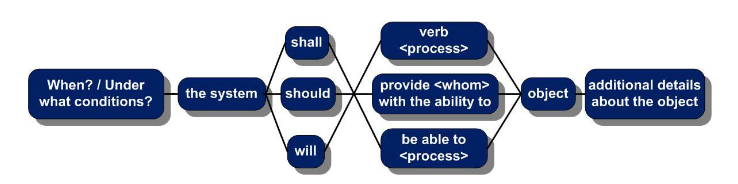
\includegraphics[width=\textwidth]{./img/introduction_req_template.PNG}\label{fig:req_template}
    \caption{Requirement formulation template.}
\end{figure}
\subsection{Requirement software}
In a complex system, there are many relationships between stakeholders and
requirements~\cite{ibm_req}. A change in one requirement may affect several other
requirements. Therefore, it is important to have a requirement software that
makes it easy to track the dependencies between the different requirements.

% More info on requirement system
\section{Shell Eco-Marathon}
Shell Eco-Marathon (http://www.shell.com/energy-and-innovation/shell-ecomarathon.html) is a yearly competition for students to compete with fuel efficient, custom made, vehicles.

There are two main class divisions, ``Prototype'' and ``Urban Concept
Vehicle''. There are also sub classes based on fuel/energy type, with a range
of fuels to choose from. Each fuel has an assigned energy value ~\cite{semrules16c1} which makes different fuel types comparable. 

\subsection{London Track}
All vehicles drive the same amount of laps, 8 in 2016 (TODO ref to rules), which equals 17.9 kilometres. Compared to earlier tracks the London track has a steeper height profile. To climb the steepest part of the track the vehicles must deliver larger amounts of torque than previous years (this is true for Elba). The height profile of the track can be seen in Figure \ref{fig:introduction_londontrack}.

\begin{figure}[H]
    \label{fig:introduction_londontrack}
    \centering
    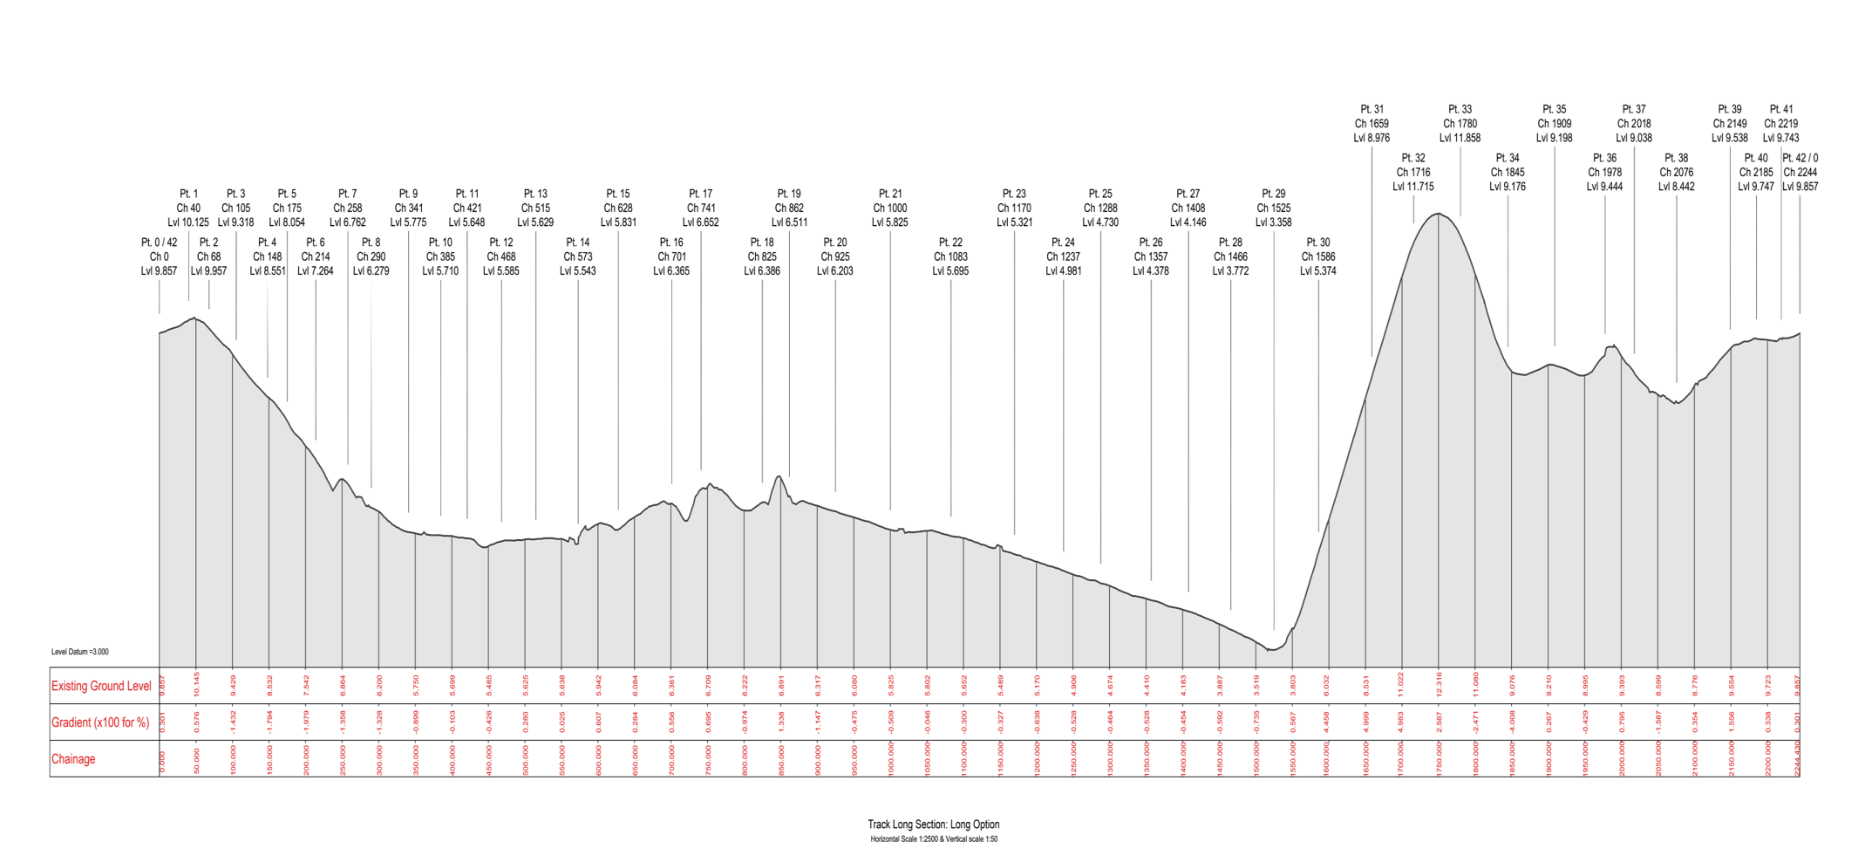
\includegraphics[width=\textwidth]{./img/introduction_londontrack.png}
    \caption{Height profile of the London track.}
\end{figure}

\subsection{Inspections}
Before any vehicle is allowed on the track it must first pass two inspections, the safety inspection and the technical inspection.

The safety inspection covers issues related to the safety of the driver and personnel and surrounding cars. 

The technical inspection covers the vehicle compliance to the rules, specifically energy usage. This ensures that the car does not use power from the auxiliary power-source to propel the vehicle in any way.

Simply passing these inspections is the main goal for many of the teams attending SEM (if the car does not change it is simpler to make the car race the next year TODO fix engrish).

%\chapter{Purpose}

Why is is this project even interesting?

Lowering fuel consumption is one of the main challenges for the automotive 
industry. Regularly new standards for permitted emissions are passed and  
one solution is to burn less fuel, which results in less emissions.

Hybrid vehicles have been growing in popularity over the last decade and 
more lately have the plug in hybrids emerged. These cars allows one 
to charge the car with electrical energy at home, potentially at a low price.

Elba can be called a plug in hybrid and reducing fuel (and energy) consumption is the goal
of SEM\@. But since the style of hybrid is very unique, with the triple motor/ engine
combination, the problem of reducing the fuel consumption is not trivial. 

\section{The Problem}
When driving any car around a track some parameters and variables have a large effect of
how much energy is used to propel the car forwards. Speed, weight, drag and friction are
the first that comes into mind. Both drag and friction are increased with speed.

\section{Applications}

\chapter{Elba The Car}

%Introduction
\section{Introduction}
Elba is the name of one of the two cars of the Eco Cars project housed by
ITRL\@.  Elba is an UrbanConcept Vehicle and have been a continuous
project ongoing for many years. The design and propulsion system, along with the
name of the UCV of Eco Cars have changed over the years and Elba is the name of
the current active car. In difference to a couple of years ago when Elba was
purely driven by an electric motor, is Elba today propelled by a parallel
electric-ethanol hybrid. The platform has been continuously improved and altered
to become the complex hybrid that exist today. The goal of Elba is to
participate in the Shell Eco-marathon.

\subsection{Propulsion}
Elba combines two electrical
motors and one internal combustion engine (ICE). The electrical motors are one
200 W direct current (DC) motor connected directly to the drive shaft and one
1.1 kW brushless DC motor (BLDC) connected via the clutch to the drive shaft.
The one-cylinder four-stroke ethanol powered ICE is connected to the drive
shaft via the clutch. These three provide a driving torque to the rear drive
shaft. The drive shaft is then connected to the right rear wheel via an 1:10
ratio planetary gear. The car fits a single human and he or she is also the
driver. The driver steers the car manually and decides upon a reference speed
that the car should follow and has the option to decide what motor/engine
combination that should be used at a specific time.

\subsection{State at start of project}
The car was in working condition when the project started, but had several
problems, including that the clutch was slow and unreliable, the overall power
output might not have been enough to be efficient on the new track, none of the
potential drivers would fit in the driver compartment and the horn disturbed the
entire electrical system.  These issues where, together with the competition
rules, the primary base for the decisions that where taken and related to the
car. Some of the work done to correct these problems where a matter of reshape
some metal piece and bolting it back in the car so that the driver could reach
the brakes. While other required an entire team of people to get a new, working,
ethanol engine in the car.

%System Overview
\section{System Overview}
\subsection{Electronic Control Units}
The car has four electronic control units (ECUs) that are responsible for
controlling different parts of the car. An overview of the communication between
the ECUs can be seen in Figure~\ref{fig:communication_overview}
\begin{figure}[H]
    \centering
    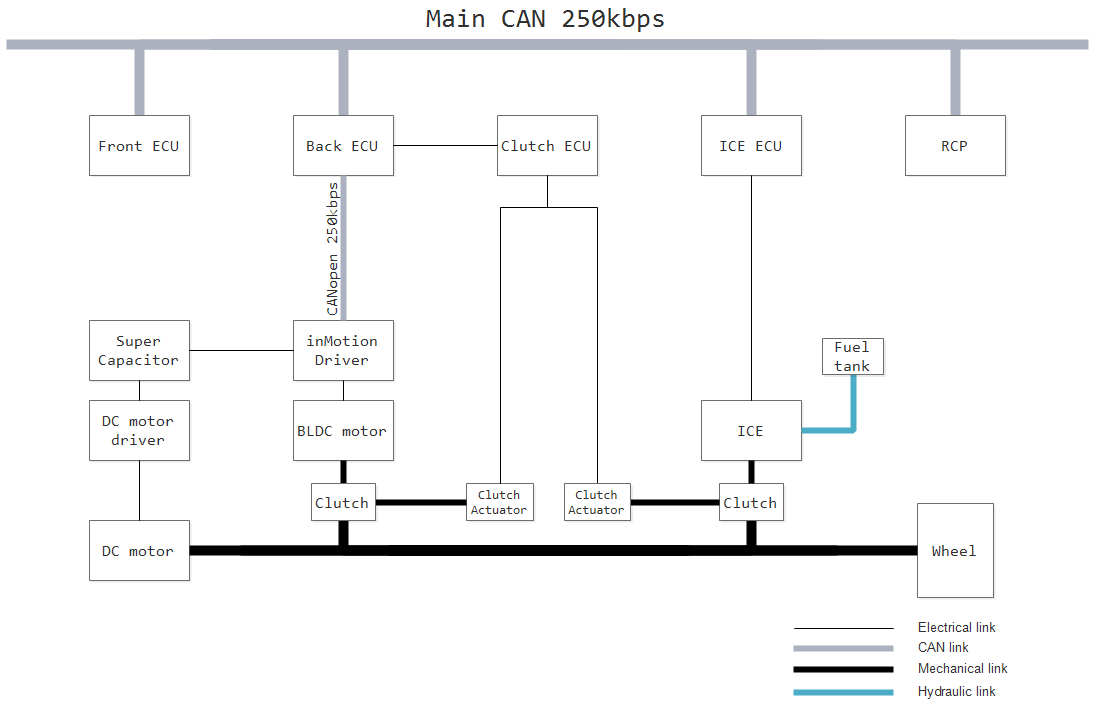
\includegraphics[width=1\textwidth]{./img/elba_communication_overview}
    \caption{Overview of the communication system and drivetrain in
    Elba}\label{fig:communication_overview}
\end{figure}
The Front ECU is responsible for the human user interface, the buttons where the
driver is able to decide drive mode and reference speed if the car is in manual
mode. It transmits speed and drive mode on the CAN bus.\\
The Back ECU controls the two motors via separate motor controllers. It has
veto over the ICE and Clutch.\\
The internal combustion engine is controlled by the ICE ECU and this is its sole
purpose, it does nothing else. It reads the lambda sensor and motor
temperature sensors to control the fuel injection.\\
The Clutch ECU controls the clutch. It interfaces to two H-bridges which in turn
steers the linear actuators.  

\subsection{Communication}
The car uses a CAN network to communicate between the distributed
micro-controllers. Any data that is needed elsewhere is sent on the CAN-bus.
Each CAN message consists of a CAN id, a 32 bit upper data integer and a 32 bit
lower data integer. Messages sent from Front ECU are sent with id 170, from
Back ECU with id 169, and from ICE ECU with id 114. GPS data from the
data-logger/GPS-unit Race Capture Pro are sent with id 180. Data position in
the messages on the CAN-bus can be seen in table REF, counting the lowest bit
as bit 1. The lower data counts for bit position 1--32 and upper data 33--64.
micro-controllers. Any data that is needed elsewhere is sent on the CAN-bus.
Each CAN message consists of a CAN id, a 32 bit upper data integer and a 32 bit
lower data integer. Messages sent from Front ECU are sent with id 170, from Back
ECU with id 169 and 113, and from ICE ECU with id 114. GPS data from the
data-logger/GPS-unit Race Capture Pro are sent with id 180. Data position in the
messages on the CAN-bus can be seen in table~\ref{table:CAN}, counting the
least significant bit as bit 1. The lower data accounts for bit
position 1--32 and upper data 33--64.
\begin{table}[H]
    \caption{Data position in different CAN messages on the CAN
    bus.}\label{table:CAN}
    \begin{center}
        \begin{tabular}{lcl}
            \textbf{Data} & \textbf{Id} & \textbf{Bits}\\
            \toprule
            Reference Speed & 170 & 1--16 \\
            Brake & 170 & 17 \\
            Reference Mode & 170 & 20--23 \\
            Auto & 170 & 24 \\
            Current Speed & 169 & 1--16 \\
            Supercapacitor Voltage & 169 & 17--32 \\ 
            Current Mode & 169 & 33--36 \\ 
            BLDC motor current & 169 & 37--48 \\
            Distance & 169 & 49--64 \\
            ICE RPM & 114 & 1--16 \\
            ICE on/off & 113 & 1--2 \\
            Fuel injection time & 114 & 17--32 \\
            GPS longitude & 180 & 1--32 \\ 
            GPS latitude & 180 & 33--64 \\
            \bottomrule
        \end{tabular}
    \end{center}
\end{table}
Another CAN network is used between the Back-ECU and the inMotion driver that
controls the BLDC motor. This network uses the protocol CANopen that
lies on top of the CAN bus. The instrumentation panel communicates via Bluetooth
with the RCP2.

\subsection{Energy supply}
All energy used to propel the car forwards (during the competition) comes from
the ethanol fuel, but electrical energy can be stored in the super-capacitor.
When the electrical motors generate energy it can be stored in this
super-capacitor for later use. The car can only start from standstill using one
of the electrical motors with energy from the super-capacitor.  

%Software and Simulation
\section{Software and Simulation Models}
Using Model Based Development (MDB), relies on verified systems models on various
levels. Elba benefits form a full system model to simulate fuel efficiency and
each ECU have a corresponding Simulink model from which all code is compiled.

\subsection{Plant Model}
The Simulink plant model is supposed to be a full system model capable of
estimating fuel consumption over an entire SEM attempt. When any component,
which has an effect on propulsion, is changed on the car the plant model must
also be updated. Naturally the goal with MBD is that any change can be simulated
with the plant model, approved and then the car is updated. But not all
simulations can be done beforehand, which was the case for the new ICE\@. 

The plant model is functionally very similar to the old model described
in~\cite{elba2015}. The structure of the model was improved to give a clearer
view, a way of including the track profile was added and errors in some models
were corrected. Also, the work of~\citep{liu2016} was included in the form of a
reference speed lookup table. The plant model also includes a model of the
testrig to simulate forces and torques it is required to output.

Since the new ICE couldn't be properly mapped, the plant model uses parameters
for the old ICE\@. This needs to be considered when interpreting results from
simulations on the plant model.

\subsection{ECU software}
All ECUs use Arduino (Due or Mega) micro-controllers, which Simulink has
compiler support for. This means that Simulink models can be compiled and
uploaded to the Arduino directly from Simulink. The Simulink to Arduino coupling
also gives the option of running ``external mode'' a Hardware in the loop type
compile mode.  This makes it possible to look at values and signals, running on
the ECU, in real-time.

%Data logging
\section{Data logging} 
The need for collecting data a very important aspect when
it comes to iteration during the development of the car. In order to determine
if changes make the car perform and handle better there is a real need for
comparing data.  In Elbas case is logging data from multiple ECU's is a must in
order to have a complete picture of the car. The absolute best way to log all
the relevant data is to log the CAN-bus. All the information sent on CAN is
relevant and of highest interest. There was always the possibility of having the
laptop in the car while driving but this didn't seem to be the best way. After
experimenting with different solutions, including making our own logging device,
was the Race Capture Pro 2 (RCP2) found to meet the requirements,
see Appendix~\ref{app:RCP}. It has the possibility to communicate with two CAN-channels
and logging different custom identifiers as virtual channels. With it's eight
analogue input channels and three digital I/O channels it is also very suitable
for logging both analogue and digital signals, which is a really good addition.

\subsection{RaceCapture Pro 2}
The RCP2 is a customizable lap timer, data logger and telemetry system designed
for racing cars. The RCP2 comes with a software GUI that is used for
configuration and this software also holds the interface for scripting
configurations.  The language used in the RCP2 is Lua and this can used to
configure everything in the RCP2. One of the two CAN channels of the RCP2 is
connected to the main CAN-bus of Elba, as can be seen in
Figure~\ref{fig:communication_overview}.  The main purpose of the RCP2 is to log
data, both data communicated on the CAN bus and the GPS-position from the dongle that
was provided. To be able to log the custom CAN-bus, there is a function called
virtual channels, this allows for customized CAN id's to be logged. There is
currently three different virtual channels that have been set up lo log messages
sent from the back, front and ICE ECU\@. These three virtual channels is logging
messages with ID 114, 169 and 170, and what is sent with these messages can be
seen in Table~\ref{table:CAN}. The exact characteristics of the \\
Besides the logging function, the RCP2 is used to track Elbas position on the
track. This is done by a GPS-dongle that was provided with the RCP2 and have the
following specifications,
\begin{align}
   CEP&=2.5\textnormal{m}\\
   R_{sample}&=50\textnormal{Hz}.
\end{align}
More on how the GPS signal is used to position Elba on the track can be found in
Section~\ref{sec:opt_pos_recon}.\\
The logging file that the RCP2 produces is a Comma Seperated Value file, even
though the file format is not standardized, there is a wide spread when it
comes to log-files, database information, serial data streams etc.
The file format is very convinient for usage with MATLAB, as there is built in
functions to load the CSV file and extracting information can be done with
minimal effort. During the project a MATLAB script have been developed to both
extract the right information and plot the interesting data. The exact way the
RCP2 loggs data can be found at~\cite{RCP2_log} 

%Requirements
\section{Requirements}
All vehicles at Shell Eco Marathon must pass two inspections before the vehicle
is allowed to enter the track. The first a safety inspection evaluating if it's
dangerous to have the vehicle on the track, both for the driver and other
vehicles. The second is a technical inspection asserting if the vehicle complies
with the competition rules and regulations.  These two inspections have been the
requirements for Elba and a lot of work have been conducted in order to make
sure that these have been fulfilled. The requirements have been something that
each respective subgroup have worked with to ensure compliance at all levels.
The requirements bellow is those that have been relevant for the current project
to work with. Requirements that have been decided by prior teams have not been
considered to the same extent since many of the vehicle design requirements
etc.\ have been considered by prior teams.

\subsection{SEM requirements}
The requirements can be found in its full length in~\cite{semrules16c1}, where
the requirements is listed with a header called \textit{Article} with a
number of sub requirements listed below. The Articles mentioned below is the
same Articles as in~\cite{semrules16c1} and the letters a, b etc.\ is each
Articles sub requirement.

hej hej hej

\begin{enumerate}
    \item Article 25
    \begin{enumerate}[label= (\alph*), leftmargin=2\parindent]
        \setcounter{enumi}{4}
        \item beeen §
        \item cool
    \end{enumerate}
\end{enumerate}
%Design Decisions
\section{Design decisions}
\subsection{Clutch decisions}
%1. What the old team told us
%2. What we told MD to do
%3. What MD did
%4. Problems still
%5. Finding the problem
%6. Fixing the arms

One of the major problems with the car have been the clutch.
Figure~\ref{fig:Drivetrain} illustrates the mechanical components of the
drivetrain of Elba.

\begin{figure}[H]
    \centering
    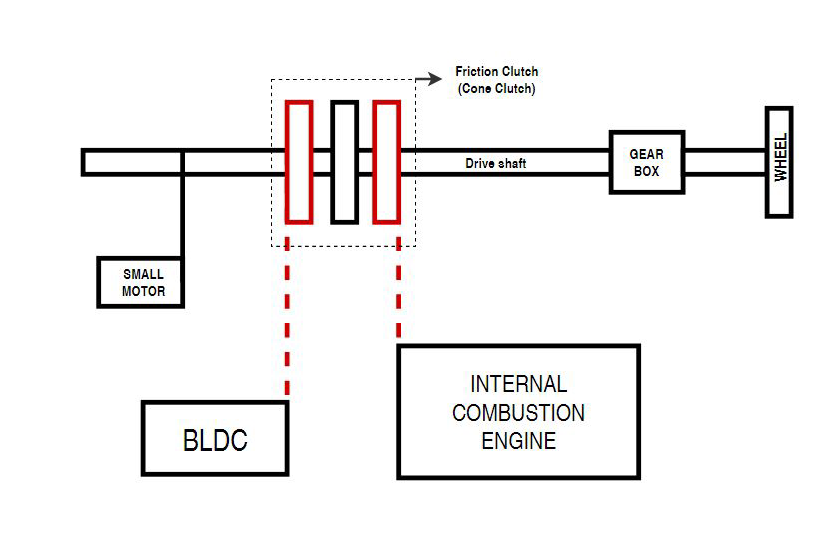
\includegraphics[width=1\textwidth]{./img/Drivetrain}
    \caption{Illustration of the mechanical components of the drive train, where
    the red plates can move towards the center plate to engage and disengage the
    motors to the drive shaft.}\label{fig:Drivetrain}
\end{figure}
At the start of the project was the problem that the clutch actuators were
oversized and thus giving more force than necessary for the clutch to engage
properly. When the clutch was engaged, there was too much actuator force, and so
the clutch plate on the ICE side got stuck center plate and could not be
disengaged using the actuator.

To solve the mechanical problems it was decided to appoint one team from the
machine design department to work solely on the mechanical parts of the clutch.
The Mechatronics team decided to completely remake the clutch ECU to make it
more robust. Despite the new ECU and the work performed by the machine design
team, which can be read about in Appendix~\cite{MD_report}, there was problems
with the clutch when it was time to race. The problems was of the same
mechanical nature as before the rework, where the clutch plate on the ICE side
could not be disengaged from the drive train. To solve this problem, several
solutions have been investigated. The clutch mechanism has been controlled by
time rather than position. One approach was to use the built in hall sensor in
the actuator to control the position. One other idea was to use an external
current sensor on the clutch ECU to control the position. A third idea was to
continue using time as reference, but increase it so that an end position is
always reached, which can be used as a reference position.

When investigating alternative three above using longer time to engage and
disengage the clutch a new problem was discovered. It appeared that even though
the clutch was not stuck to the center plate it still could not be properly
disengaged. This was due to the geometry of the lever arm which pushes the
clutch plate.  After this important insight the drive train was disassembled and
new lever arms were constructed and manufactured. When the drive train was
assembled again the clutch worked like expected. Figure~\ref{fig:clutch}
and~\ref{fig:old_clutch} shows both the new and old lever arms.

\begin{figure}[H]
    \centering
    \begin{subfigure}[H]{0.55\textwidth}
    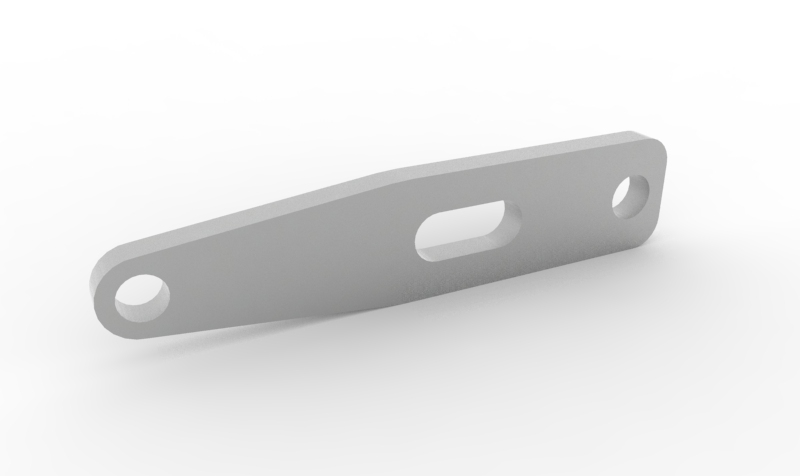
\includegraphics[width=\textwidth]{./img/clutch}
    \caption{The new clutch lever arms}\label{fig:clutch}
    \end{subfigure}
    \begin{subfigure}[H]{0.44\textwidth}
    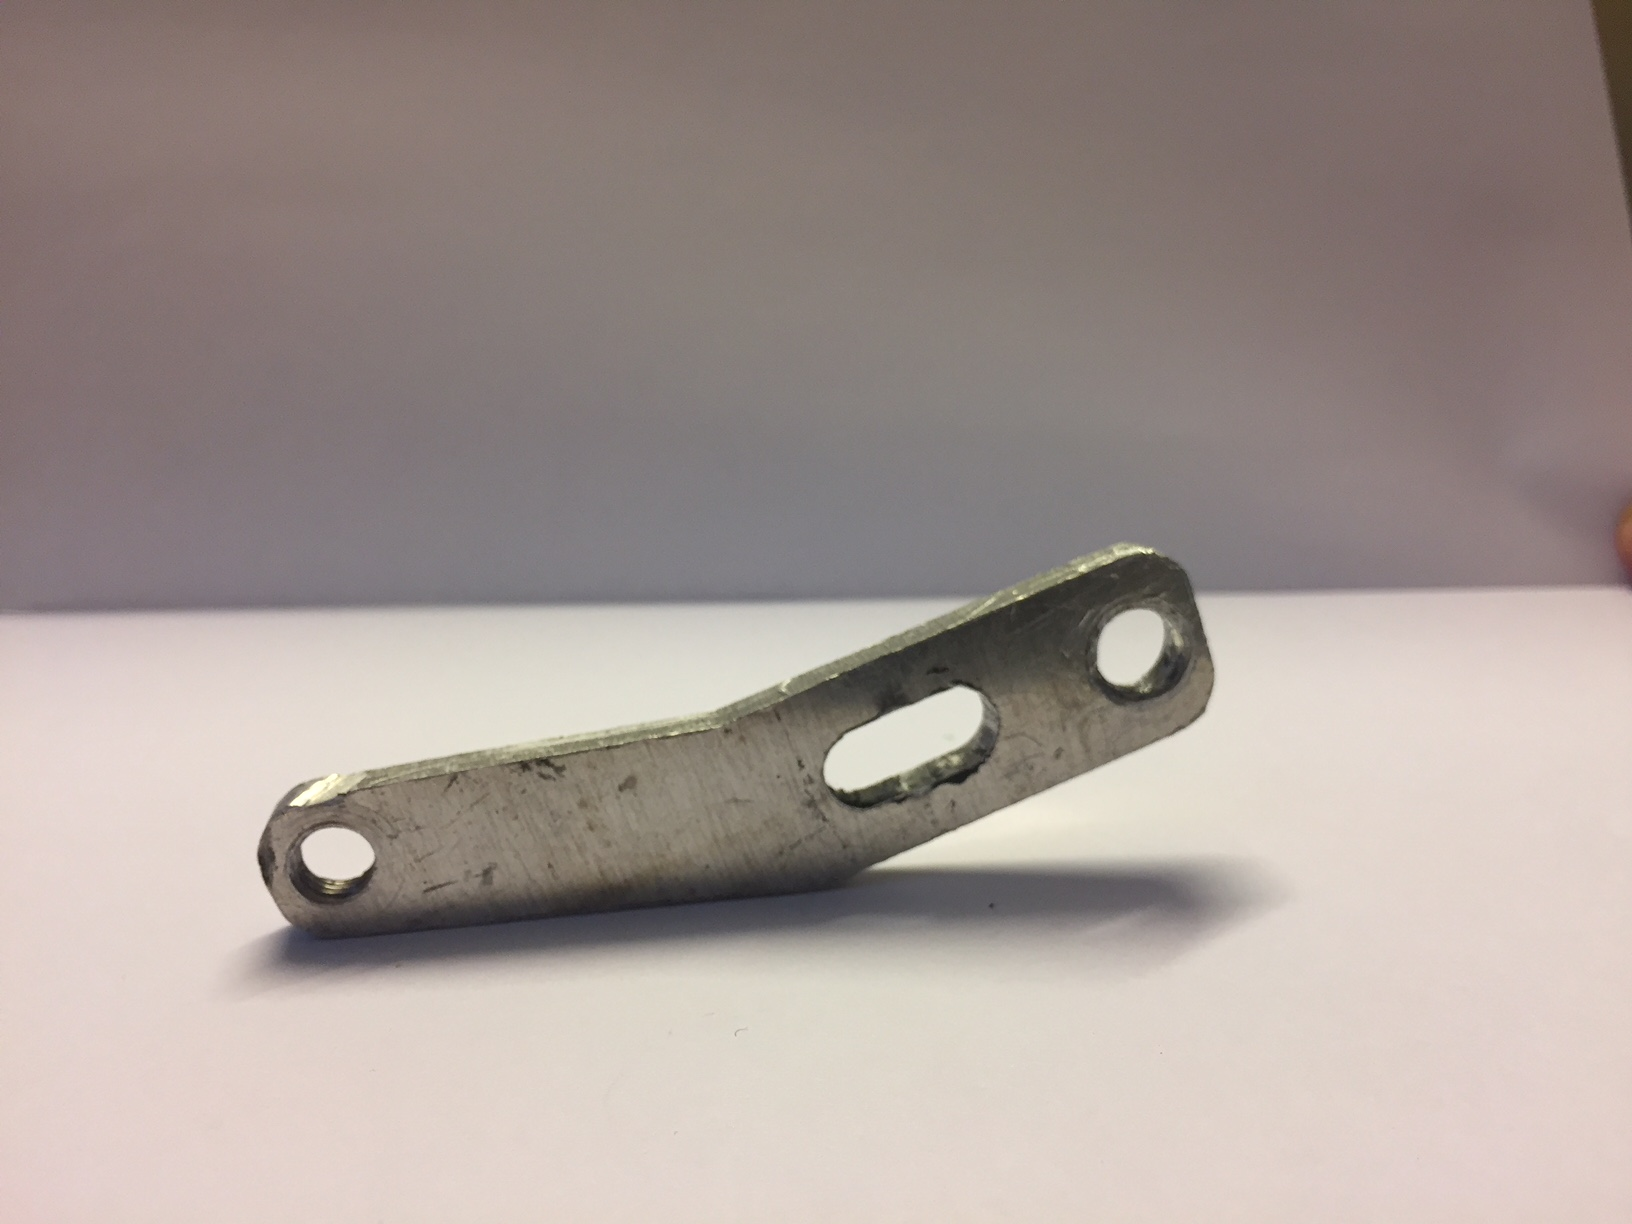
\includegraphics[width=\textwidth]{./img/Clutch_old}
    \caption{The old clutch lever arms}\label{fig:old_clutch}
    \end{subfigure}
    \caption{This image shows the difference between the old and the new lever arms that are used to push the clutch plates.}
\end{figure}

\begin{figure}[H]
    \centering
    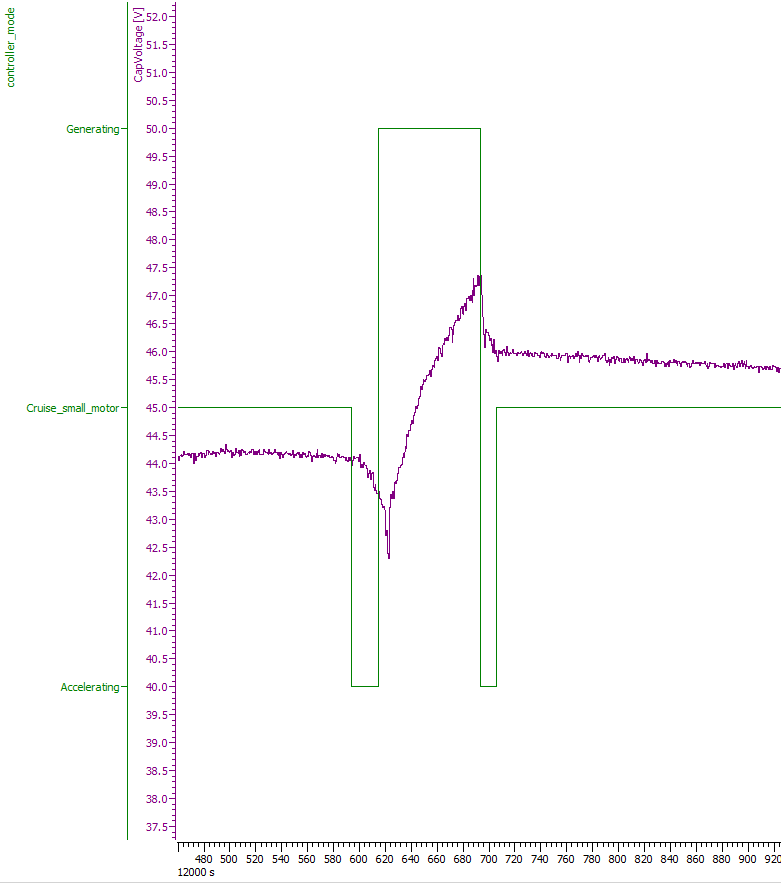
\includegraphics[width=0.75\textwidth]{./img/elba_capvoltage_regen}
    \caption{Capacitor voltage and drivemode as a function of time}\label{fig:elba_capvoltage_regen}
\end{figure}

Figure~\ref{fig:elba_capvoltage_regen} illustrates a sequence from CANoe where
the capacitor is charged by changing mode from the small DC motor when the
voltage is low and charging to a higher voltage level then changing back to the
small DC motor.

\subsection{Internal Combustion Engine and ICE ECU}
One of the requirements from the ICE-department was that the ICE should be run
on ethanol. An engine running on ethanol needs to have a higher compression ratio
than a petrol engine~\cite[p.8]{ICE_report}.
The requirements engineering and modifications on the new ICE was set by the ICE
team based on the requirement given in the rules, along with recommendations from 
previous year. 


It had been said that last years ICE where too powerful, when the car regenerated its
maximum energy at the average track speed the car still wanted to accelerate. 
<<<<<<< HEAD
Going faster than required is saves time but is a waste of energy and therefore
bad at SEM\@.
A new ICE was puposes with 50 cc compared to earlier 57 cc. Vinkelväxel blä. 
=======
Going faster than required is saves time but is a waste of energy and therefore bad at SEM.
A new ICE was proposed with 50 cc compared to earlier 57 cc. Another major difference 
was that the new motor had an horizontal output shaft compared a vertical one. 
This meant that no bevel gear had to be used, which was a major point of failure earlier.
The ICE had to be shipped relatively fast and a requirement from ICE-group supervisor was that 3 identical engines had to be bought. This limited the choice even further. 
Which motor that was chosen in the end and why is motivated in greater detail in appended paper \citep{ICE_report}.
>>>>>>> 981c94933f27e264bf381d73ab438a42118ecbb7

To control the new engine, a new ICE ECU was needed. It was also decided
that the new ICE ECU would contain more sensor inputs as well as the possibility
to control the ICE ignition. All functionality of the old ICE ECU would still be
present, namely:
\begin{itemize}
    \item Simulink TLC software.
    \item Feedback control loop of injection time.
    \item Lambda value sensing.
    \item Encoder reading with index pulse from ICE\@.
\end{itemize}
More sensor data together with ignition control would give possibilities
for more exact control of the ICE\@. The extra features of the new ECU were:
\begin{itemize}
    \item Motor oil temperature sensing.
    \item Ambient air temperature sensing.
    \item Ignition control.
\end{itemize}
The features were implemented on the ECU PCB and the system was designed so that
the sensors and features could be implemented incrementally according to the
time and need of the project. Given that the amount of time that would be needed
to get the car in working condition before the race was not easily planned
beforehand, it was beneficial to have a base functionality with flexibility to
add features.

\subsection{Door}
The car is required to have a door, with a large enough entrance and working
locking mechanism~\cite{semrules16c1}. Since the old, layered carbon fibre door
was too flimsy and also back hinged (there is a reason its called ``suicide door''),
it was decided a new, sturdier, door would be made. Two lightweight-construction
student took this upon them self as a bachelors project. 

The new door where constructed in a carbon fibre sandwich style and was open in
a scissor manner. The door became sturdier but the hinges where less than ideal
and the closing mechanism did not work.

%Results
\section{Results}

\subsection{Competition}
At the time the team arrived in London the ICE had never been started with only
ethanol as fuel, the door had to be mounted and the team needed to do a number
of small changes to be able to pass both inspections. Most time was spent to get
the engine running, but it was never able to run for more than a couple of
strokes. 

Both the technical inspection and safety inspection were passed. There where a
few complaints: The doors closing mechanism was insufficient, the indicator
lights were to weak, and the fire-extinguishers expirations date had passed.
All these had to be reinspected before Elba was given a pass.

It was decided that one attempt should be made even if the engine never had been
started properly. Since the car must be rolling to start the ICE the inertia of
the car will keep the ICE turning even if it misfires (the wheel inertia is not
enough for this). This meant that the ICE started once the car finally was
running during the attempt. %But it was soon discovered that the engine could
%not be shut off, if the clutch was disengaged the engine kept running and
%revving at dangerous levels. %KOMMENTAR: Känns som att vi kan utelämna denna
%bit... :D /Emil
At the compulsory stop after one lap the clutch to the ICE did not properly
disengage, causing Elba to stall the engine with clutch engaged. While trying to
get going again the clutch could not be disengaged and the attempt had to be
aborted.

Therefore Elba never got a competition result. 

\subsection{End of project}
%%in this section we will write what is done so far and the.

A lot has happened with Elba since the competition in June. At the end of this
project the car is finally in fully working condition. Both the clutch and the
ICE which were the major problems have been fixed to a point where they work
sufficiency, but not optimal. For the ICE it would be needed to study the engine
parameters to make it run more efficiently. The clutch is very slow and would be
much more energy efficient if it could engage and disengage much faster. One way
could be to study the actuator timings and decrease the distance that the
actuator moves, but still keep the proper functionality.

\chapter{Optimization}

%Introduction
\section{Introduction}
The main goal of the project is to have the car consume the least amount of fuel
possible.  In the ideal world shall the engines and motors therefore always
operate within a certain range of their optimal point of operation. The torque
request from each of the engine/motors should consider this in order to reduce
fuel consumption. In addition to this goal, there is a number of constraints
that needs to be considered in addition to the generic fuel consumption
optimization.  Things like track topography, super-capacitor voltage,
competitors on the track etc.\ will all weight in on the output request. The
optimization algorithm used in Elbas automatic drive mode was developed as a
part of a Master Thesis~\cite{liu2016}. The control architecture for this
optimization consists of two or three layers and the thesis have completed the
top layer speed reference control. This chapter will cover the decentralized
hierarchical predictive control that is used to calculate the speed trajectory
and it's implementation.

\section{Design Decisions}
The need for an optimization can seem obvious in order to lower fuel
consumption. However, depending on the tracks topography there might be other
areas that would need much more consideration and tings like weight, frontal
area and rolling friction might have a grater impact in some cases. In recent
years the track of SEM have been more or less flat, with only minor deviations
in altitude. With this track, the considerations for an automated drive mode
would more or less only consist of making sure that the voltage level of the
super capacitor is within it's boundaries. This means that the ICE needs to be
started when the voltage level gets too low and regenerate energy into the super
capacitor. The reason for this is that the efficiency of the electrical motors
exceeds that of the ICE, and in so it will be more efficient to drive Elba with
the electrical motors.  Once SEM moved to London, where the altitude changes of
the track is much more significant, the conditions became different. On top of
the voltage level of the super capacitor there is also room for optimizing the
torque requests so that the most efficient propulsion constellation is active at
all times. It is also nessesary to time the accessible energy so that there is
enough energy in the super capacitor in beginning of an uphill, the possibility
to regenerate from driving downhill etc.\ all added to the complexity of the
optimization.  These new levels of complexity makes the optimization become more
of an factor then previous years, and in so there was a collaboration with a
master thesis student who used Elba as an experiment in the
thesis~\cite{liu2016}.

The Simulink lookup table that was produced from~\cite{liu2016} was dependent on
the distance traveled on the track and in so there was a real need to get an
accurate position reading. There was two options, to get an GPS-positioning
device and get that to talk with the rest of the car, or to use the encoder
already mounted on the drive shaft. Both had their disadvantages, with the
encoder reading having the tendency to drift and the inaccuracy of the path
chosen on the track and the GPS with its CEP of $\pm2.5\textnormal{m}$. When the
RCP2 was bought it came with an GPS solution already implemented, this made the
choice of having both of them easier, more can be found in
Section~\ref{sec:opt_pos_recon}. The next problem arouse was to filer the
readings of both the GPS and the encoder to have a reliable positioning source.
Due to priorities and limited amounts of time, is the filtering currently not
implemented. 

\section{Constraints}
The optimization is limited by the constraints of the physical system, meaning that
the controller is not able to operate outside the limits of the system. These limits
are,
\begin{align}
    &U_{cap} \in [39,48]~\textup{V} \\
    &\nu \in [0,15]~\textup{m/s}\\
    &a_{\max} \in [-1,1]~\textup{m/s$^2$}
\end{align}
where $U_{cap}$ is the voltage level of the super-capacitor, $\nu$ is the speed
and $a$ is the acceleration in every time step. Due to the fact that there is a
lower limit to the voltage level of the super-capacitor, it is necessary to
change drive mode to engage the ICE in order to regenerate and store energy
until the upper limit is reached. Since the optimization is currently only done
in the top layer, there is a need for the voltage limit to be considered
manually in the model.

\section{Position recognition}\label{sec:opt_pos_recon}
The optimization bases the output reference speed on the current position on the
track. This yields the need for a position recognition with an accuracy precise
enough to be able filter it with sufficient results. The track itself, rather
then time is discretized in order to get a more accurate position in relation to
the tracks topography. \\
There is two ways of finding Elba's position on the track. The first way is a dead
reckoning system based on the shaft encoder~\cite[p.~49]{elba2015},
which calculates the position based on the rotational speed of the shaft. The
second way is based on the GPS system implemented in the race capture pro 2,
where the GPS signal is taken from it's raw form and reshaped with a
Lua-script\footnote{Lua is a dynamically typed scripting language, www.lua.org}
into a CAN-message that is sent on the CAN-bus.


\section{Simulink implementation}
The complete description of the algorithm is found in~\cite{liu2016} and the
implementation is based on this thesis.  There is a function for calculating the
distance traveled from the encoder, this takes the absolute dead reckoning
position calculated from the shaft encoder and an indicator for a new lap, as
input. When the indicator for a new lap is pressed, the dead reckoning position
is zeroed in the function block and the position is calculated and delivered as
the output. The position should then be sent to a Particle Filter block where
both the dead reckoning and the GPS position is inputed.  However, the Particle
Filter itself is not implemented at the moment and is considered to be something
future groups need to work on. These two positioning systems is supposed to be
used to get the estimation of the distance Elba have traveled on the track.

There are three inputs into the three dimensional optimization lookup-table, the
first one is time. This input is used to synchronize the different time scales
in the table and Simulink. The speed input is read from the CAN-bus and is the
current speed of Elba. The track position is the calculated distance traveled
on the track from the filter. The output of the block is an acceleration
reference which needs to be converted to an reference speed since Elba is
currently controlled with speed request. 

\section{Simulation}

\subsection{Static reference speed}\label{sec:opt_sim_static}
One lap around the track was simulated using the plant model with a constant reference speed of 7 m/s (the slowest allowed speed to be able to complete the race in time). %The resulting speed and vehicle height position can be seen in Figure \ref{fig:optimization_static_speed} 

%TODO: Frågan är om denna ska med alls...
%\begin{figure}[H]
%    \centering\label{fig:optimization_static_speed}
%    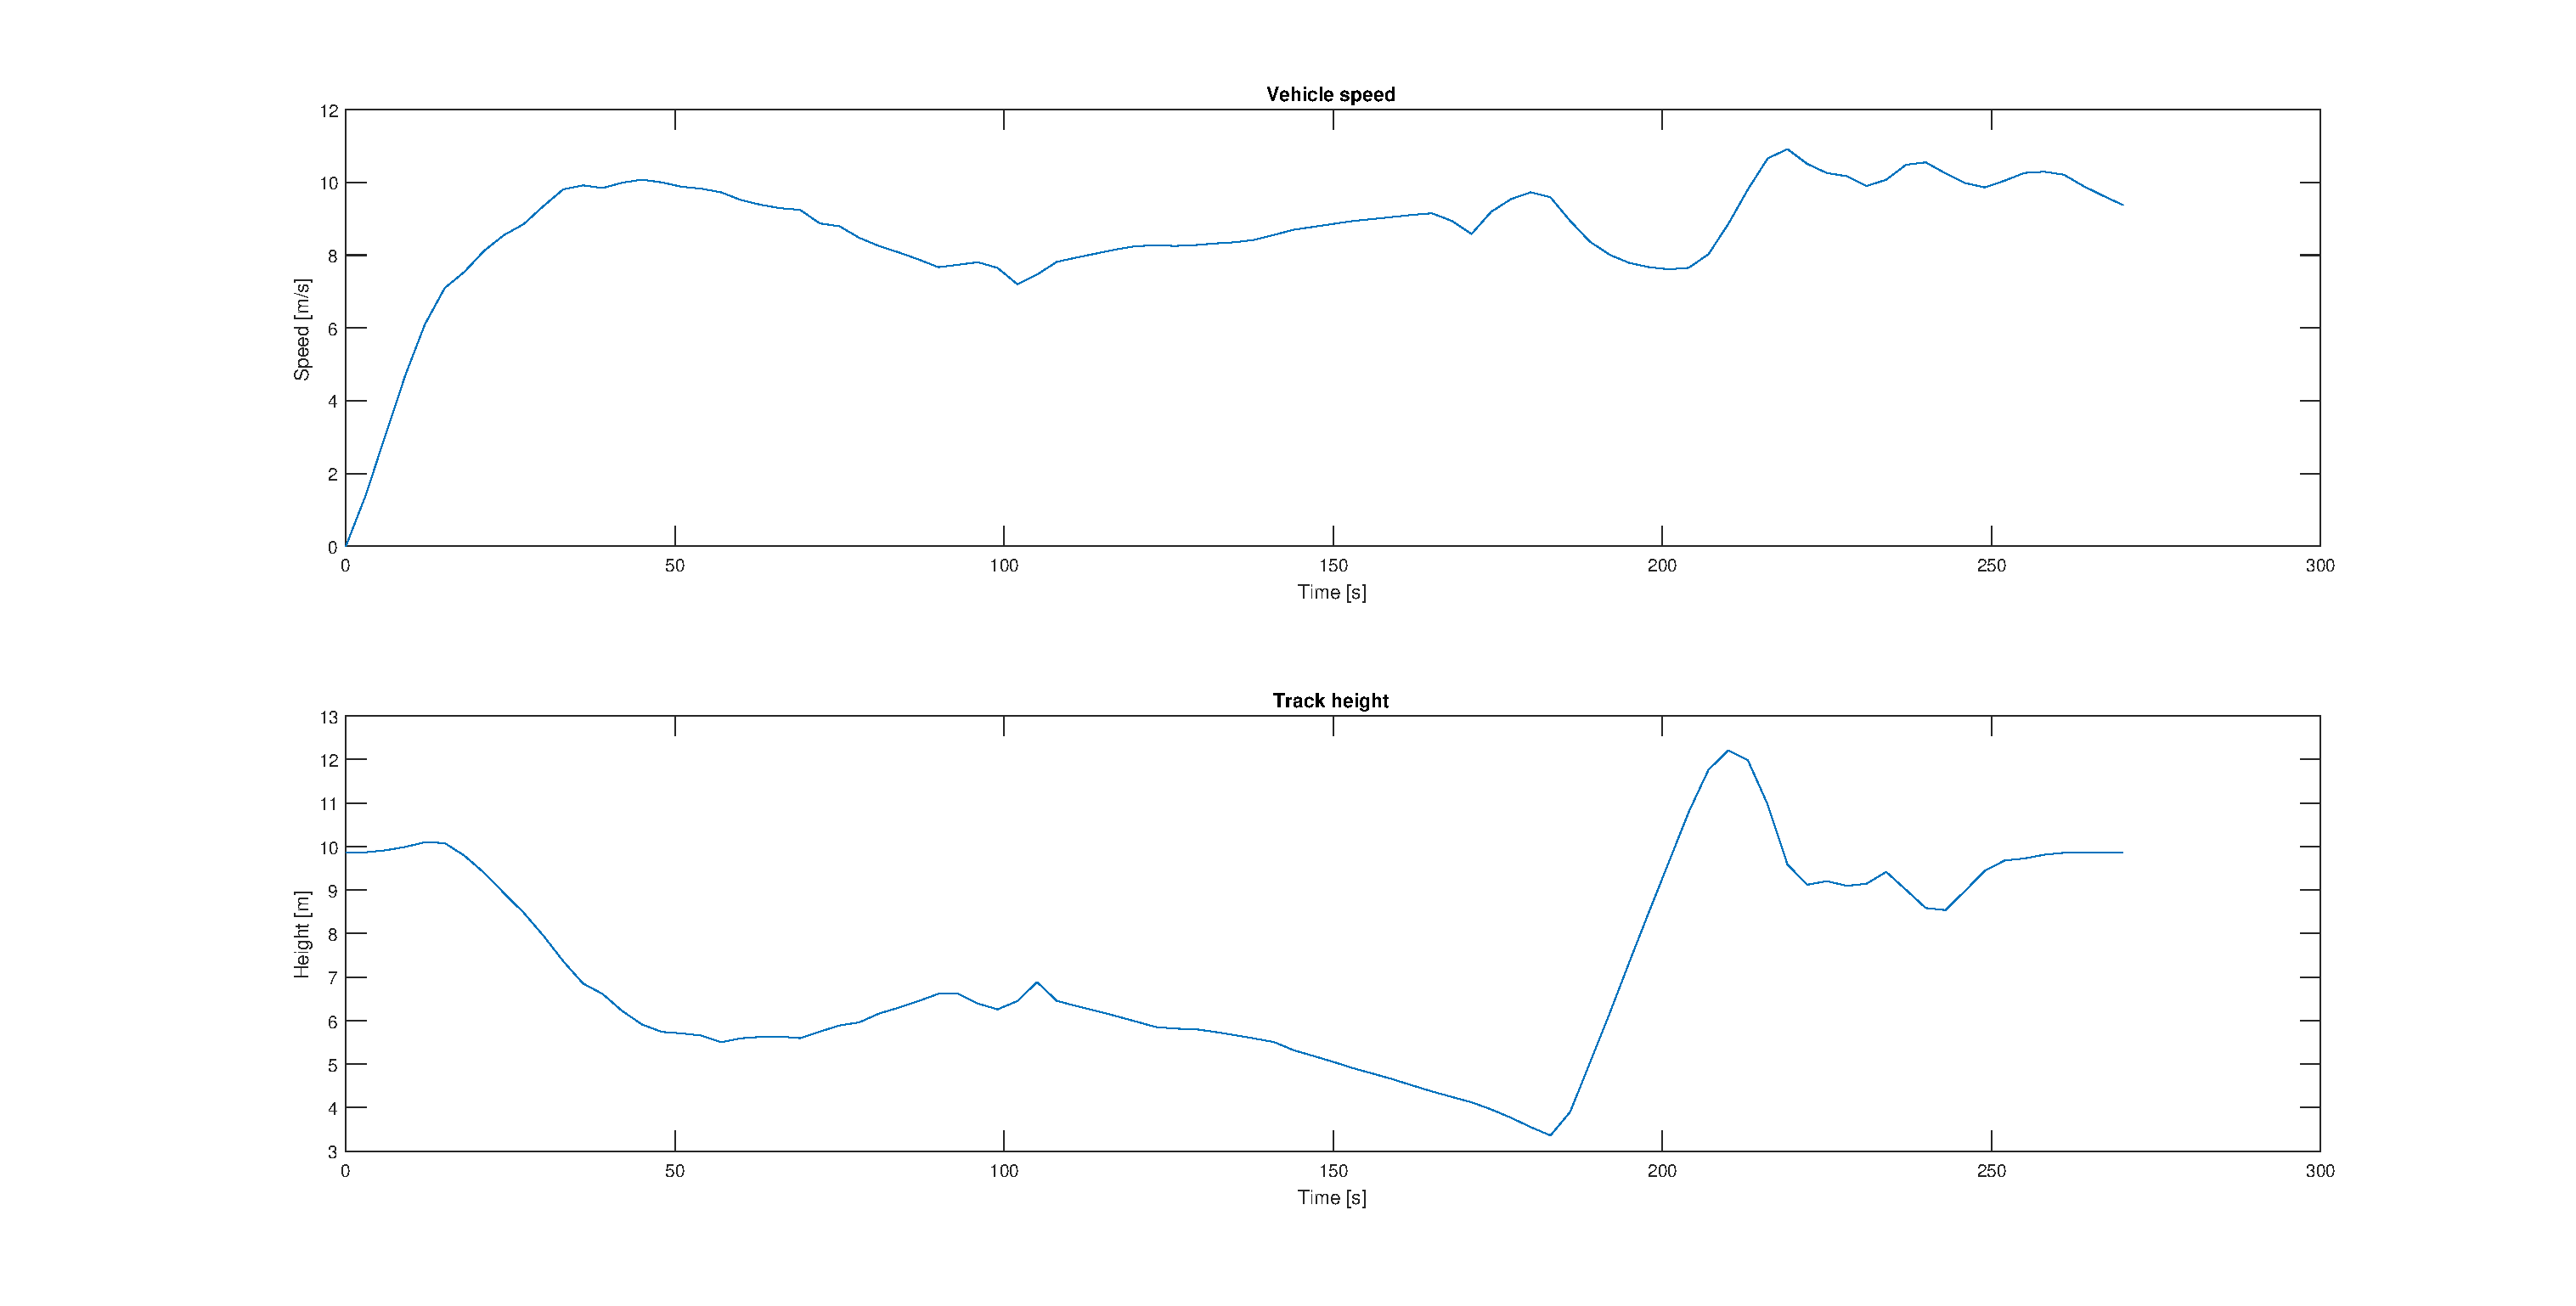
\includegraphics[width=\textwidth]{./img/optimization_static_speed.eps}
%    \caption{Plots of vehicle height and speed as a function of time.}
%\end{figure}

The fuel consumption in $\textnormal{km/l}$ fuel, $f_c$ was calculated according to

\begin{equation} \label{eq:optimization_fuelconsumption}
	f_{tot} = \frac{d_l}{f_i+f_c},
\end{equation}

where $d_l$ is the distance of one lap, $f_i$ the fuel consumed by the ICE and
$f_c$ the equivalent amount of fuel that the super capacitor has been discharged
by since the start of the race, calculated as

\begin{equation} \label{eq:optimization_ethanolenergy}
	f_c = \frac{({{u_{c_0}}^2-{u_{c_{end}}}^2})c_c}{2k},
\end{equation}

where $u_{c_0}$ is the initial capacitor voltage, $u_{c_{end}}$ is the capacitor
voltage at the end of the race, $c_c$ is the capacitance in the capacitor and
$k$ is the conversion ratio from litre ethanol to energy in joule, retrieved
from~\cite{fuelconversion}.

This resulted in $f_{tot} = 172.8$ $km/l$. %TODO: göra snyggare

\subsection{Optimized reference speed}\label{sec:opt_sim_static}
Using the optimized speed controller as a lookup table (produced by
\citep{liu2016}) dependant on vehicle speed, distance and elapsed time, a new
simulation could be produced. The resulting speed and vehicle height position
can be seen in Figure~\ref{fig:optimization_optimal_speed}

\begin{figure}[H]
    \centering
    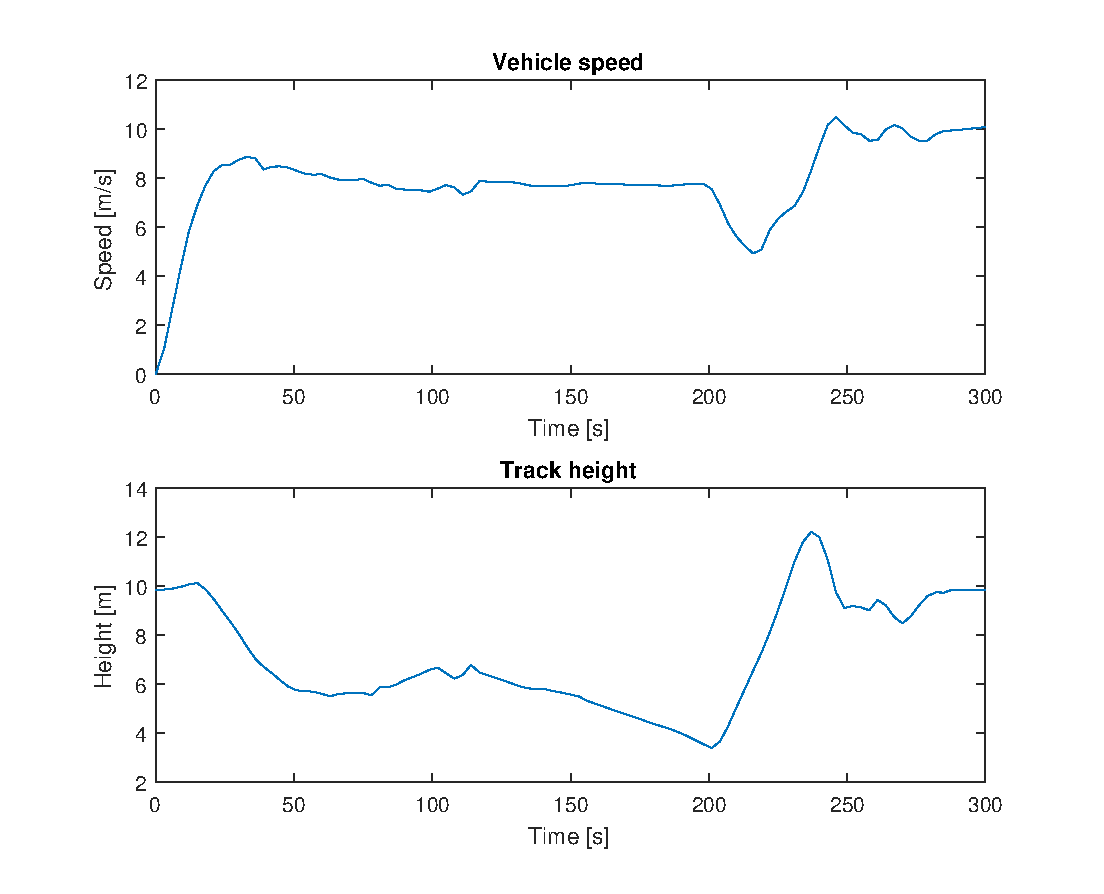
\includegraphics[width=\textwidth]{./img/optimization_optimal_speed.eps}
    \caption{Plots of vehicle height and speed as a function of
    time.}\label{fig:optimization_optimal_speed}
\end{figure}

The amount of kilometers travelled per liter fuel $f_{tot}$ was calculated
according to equation~\ref{eq:optimization_fuelconsumption}. This resulted in
$f_{tot} = 194.1$ $km/l$. %TODO: göra snyggare

\chapter{Testrig}
\section{Introduction}
When designing a complex system such as a hybrid vehicle, being able to continuously test the system is important to validate that the requirements are met and to verify the models. To be able to do a full system test, the car has to
physically run on a track. This can be cumbersome, or in the case of the London
track, impossible at times. Therefore, a test rig is designed and built. The
design process uses the V-model approach with a set of live requirements and
continuous unit and integration testing. The overall goal is to not only be able
to do a faithful simulation of the Shell Eco Marathon track in London, but to be able to
supply any track (with certain limitations on power and speed demands) to the
test rig and simulations on the car.

\section{Requirements}
The requirements on the test rig are designed to capture the essential demands
on the system. Firstly, the high level User requirements are set. These are set
to capture the problem and to describe the goal of designing the system
~\cite{ibm_req}. The User requirements are then developed into the System
requirements that describe the limitations and demands on the system and its
subsystems.

\section{Car dynamics} \label{sec:cardynamics}
The calculations in this section are in many ways the same as the calculations
given in the previous teams report in Appendix~\ref{app:elba2015}. Though some
of the equations are repetition of what was done last year, they are
done here again with some improvements and more references to make the
derivations of the equations clearer.

When simulating a track, one needs to know the force exerted by the environment
on the car. A graphical representation of the forces that act on the car is
given in Figure~\ref{fig:testrig_elbadynamics}.
\begin{figure}[H]
    % TODO: Make a better picture!
    \label{fig:testrig_elbadynamics}
    \centering
    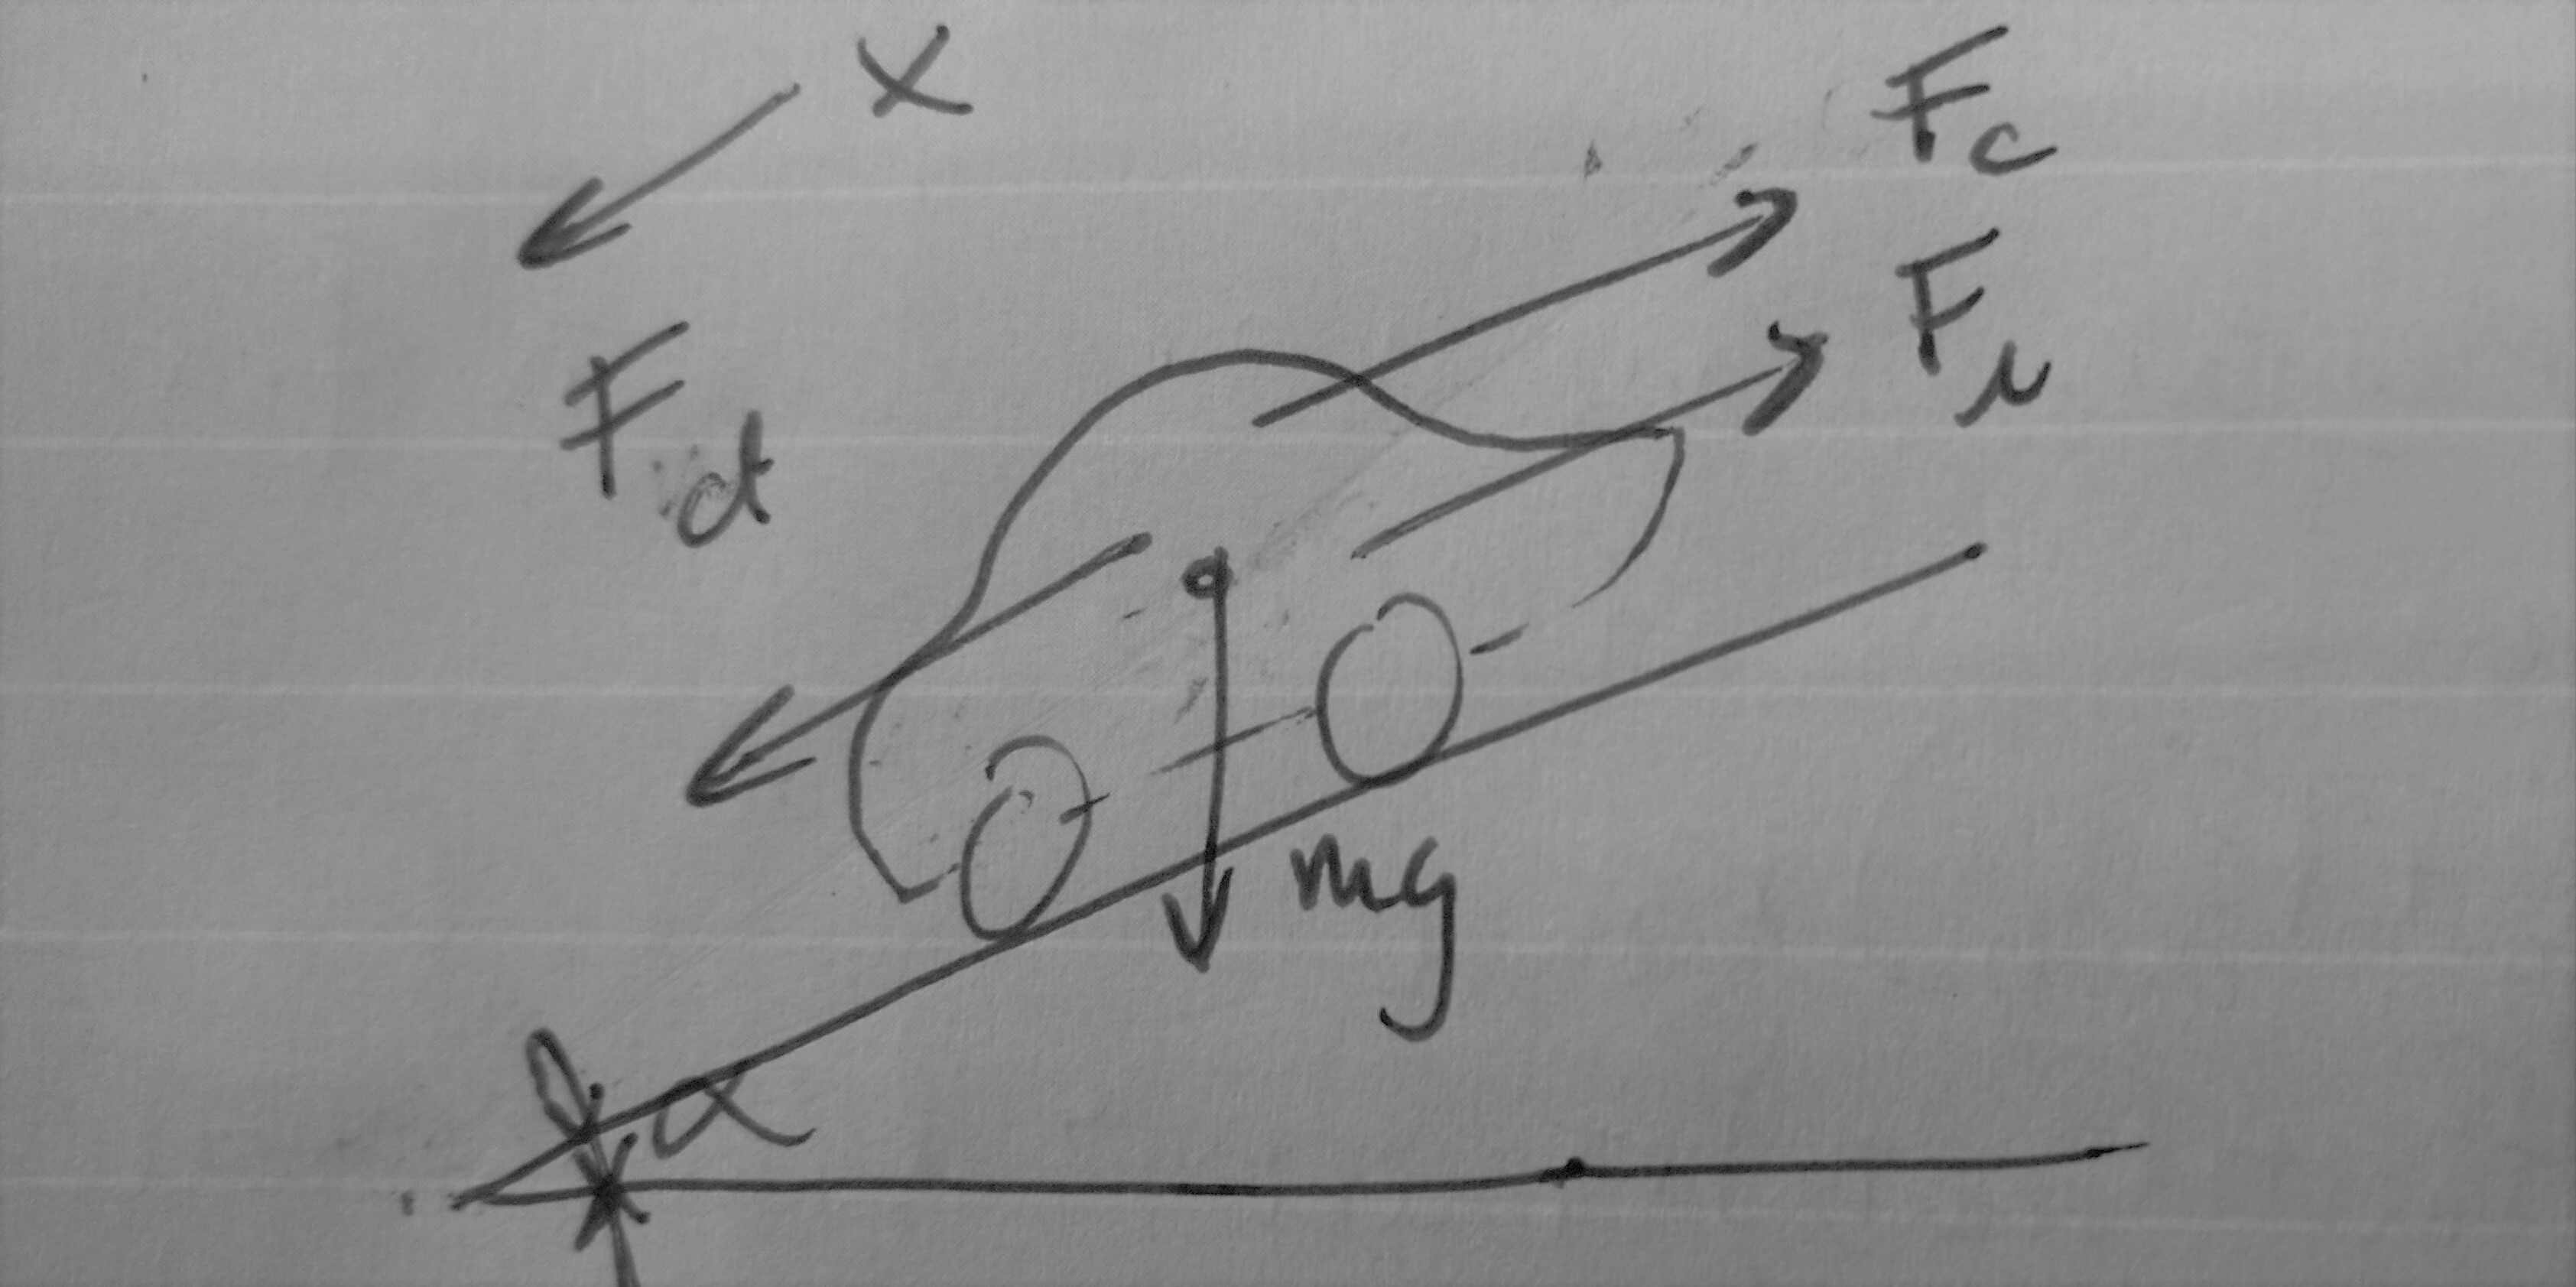
\includegraphics[width=0.5\textwidth]{./img/testrig_elbadynamics.png}
    \caption{Dynamic model of ELBA.}
\end{figure}
The motion equations on the system are 
\begin{equation} \label{eq:testrig_cardynamics}
    m\ddot{x} = F_d + mg\sin{\alpha} - F_c - F_{\mu},
\end{equation}
where $F_d$ is the effective driving force of the car, $m$ is the mass of the
car and $alpha$ is the slope from the horizontal plane. The resistance terms
$F_c$ and $F_{\mu}$ are air and road resistance, respectively. The air drag $D$
around an object can be calculated as \cite{nakayama2002}
\begin{equation} \label{eq:testrig_airdrag}
    D = C_D A \frac{\rho v^2} {2}
\end{equation}
with object velocity $v$, surface area vertical to the movement direction $A$
and air density $\rho$. Most terms in Equation~(\ref{eq:testrig_cardynamics})
are constant throughout a driving instance. Rewriting to
\begin{equation} \label{eq:testrig_csimple}
    C_{tot} = \frac{C_D A \rho} {2}
\end{equation}
yields a simplified equation that only depends on the velocity,
\begin{equation} \label{eq:drag}
    F_D = C_{tot}v^2.
\end{equation}
The total drag coefficient $C_{tot}$ will depend on the vertical area, the density of
air and the drag coefficient $C_D$. The air density is considered to be constant
and is known. The area of Elba can be estimated using simple methods. Finally,
the air drag coefficient $C_D$ is unique to each and every object and is
determined experimentally. For this project, the estimations given for a
passenger car is used. Detailed calculations and values are given in
Appendix~\ref{app:rigdata}. 

% This section is under construction. Need some reference/experiment on how to 
% model rolling friction.
The rolling friction of a car is modeled as a stepfunction, being non-zero at
all velocities that are not zero.

With the air drag, rolling friction and gravity terms known, only two terms of
Equation (\ref{eq:testrig_cardynamics}) are unknown. To fully model the cars
dynamics, the inerta term needs to be modeled. Since the weight of the vehicle
is known, $\ddot{x}$ needs to be derived for an accurate system model.
Knowing the radius of the rollers and the cars wheels, the linear acceleration
can be calculated by measuring the rotational acceleration on the roller. This
is done by an incremental encoder on the roller shaft. Rotational speed is
calculated in the microcontroller and rotational acceleration is derivated from
rotational speed. Using the roller radius, $r_{roller}$, the linear acceleration
is calculated.

Rewriting Equation (\ref{eq:}), (\ref{eq:drag}) and the friction force gives the
desired linear testrig simulation force on the right hand side,
\begin{equation} \label{eq:simulationforce}
    F_d = m\ddot{x} - mg\sin{\alpha} + C_{tot}\dot{x}^2 + F_{\mu}.
\end{equation}

Using the height profile of the London track and the plant model of Elba, $F_d$ during an entire lap could be simulated, as shown in Figure (\ref{fig:testrig_negative_forces}).

\begin{figure}[H]
    \label{fig:testrig_negative_forces}
    \centering
    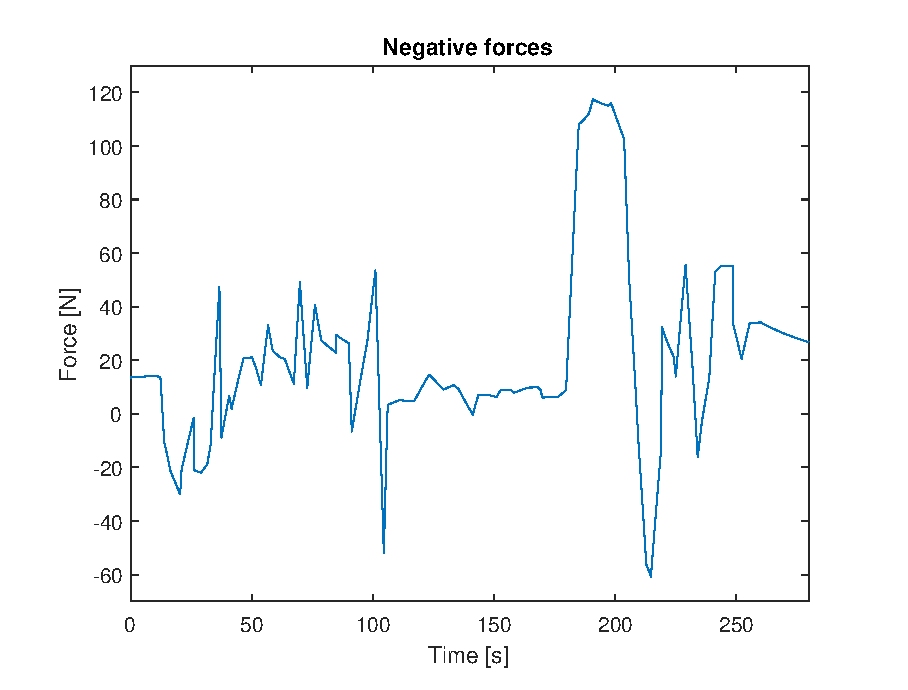
\includegraphics[width=\textwidth]{./img/testrig_negative_forces.eps}
    \caption{Negative forces acting upon Elba in one lap.}
\end{figure}

\section{Testrig dynamics}
In order to let the testrig output the correct linear force to the car, the
controller for the testrig need to know the dynamics of the testrig itself. This
is to compensate for internal frictions and inertias. The driveline of the
testrig has two separate steps, the motor and the roller, connected by a chain
gear with gear ratio $n_{chain}$. A prinicple schematic of the testrig from
motor to roller is displayed in Figure~\ref{fig:testrig_testrigdynamics}.
\begin{figure}[H]
    %TODO: Need a better picture!
    \label{fig:testrig_testrigdynamics}
    \centering
    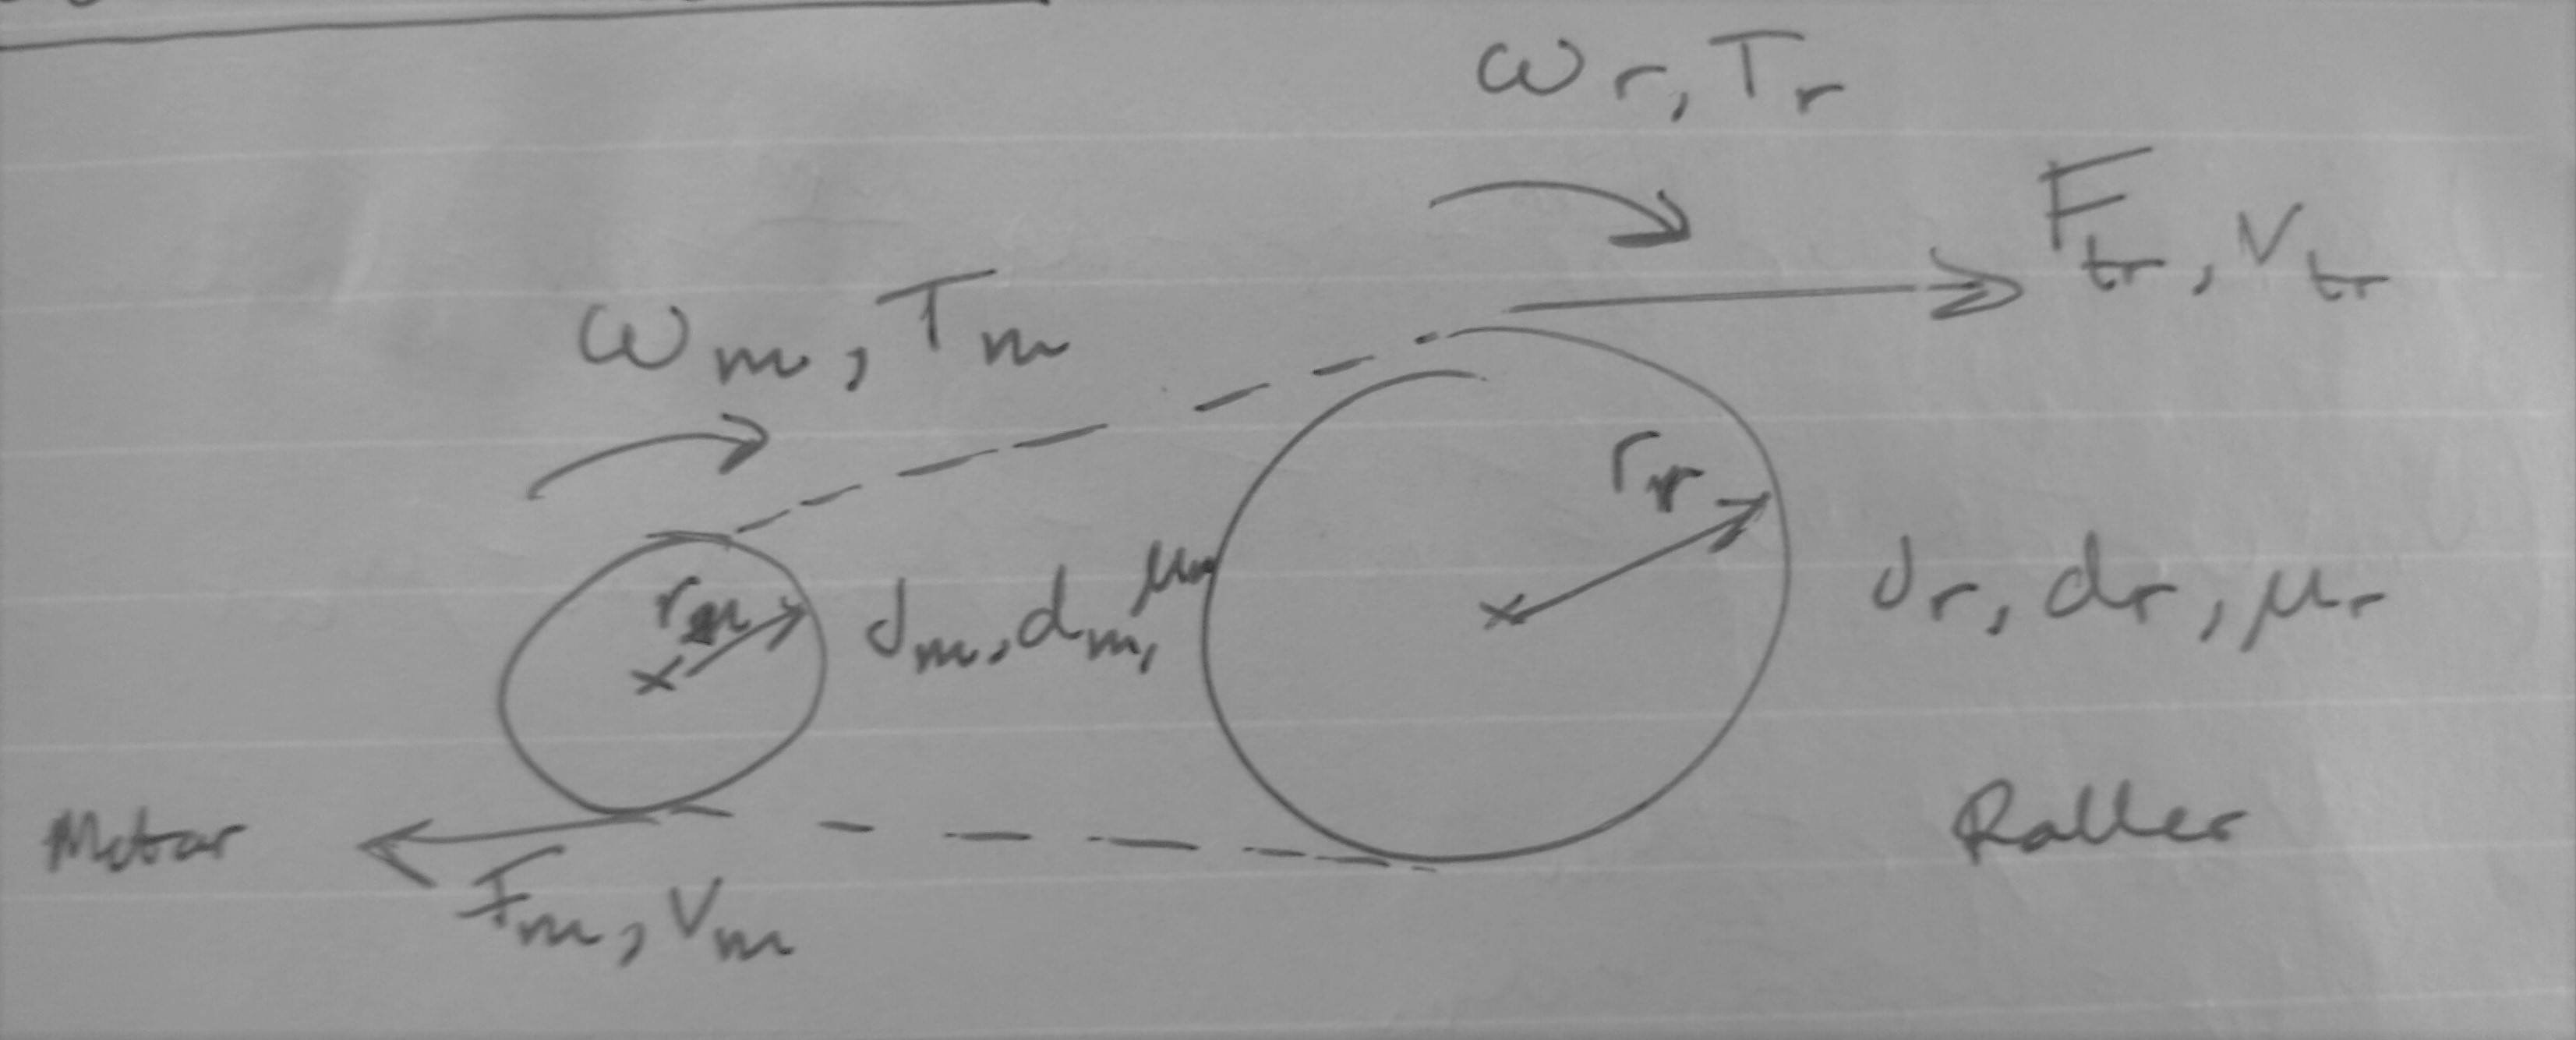
\includegraphics[width=0.9\textwidth]{./img/testrig_testrigdynamics.png}
    \caption{Principle schematic of the testrig from motor to roller.}
\end{figure}
The dynamic equations for the rollers are
\begin{equation} \label{eq:testrig_rollerdynamics}
    J_r \dot{\omega}_r = F_{tr}r_r - d_r \omega_r - \mu_r,
\end{equation}
where $J_r$ is the inertia of the rollers and $\omega_r$ is the rotational velocity
of the roller. The frictional terms are the viscous friction $d_r$ and the
constant friction $\mu_r$ which is modelled by the Karnop model (??).

Connecting the rollers and the motor is a chain gear. It is modelled as a
generic gear box. A principle drawing of it is given in
Figure~\ref{fig:testrig_chaingear}. 
\begin{figure}[H]
	%TODO: Need a better picture!
    \label{fig:testrig_chaingear}
    \centering
    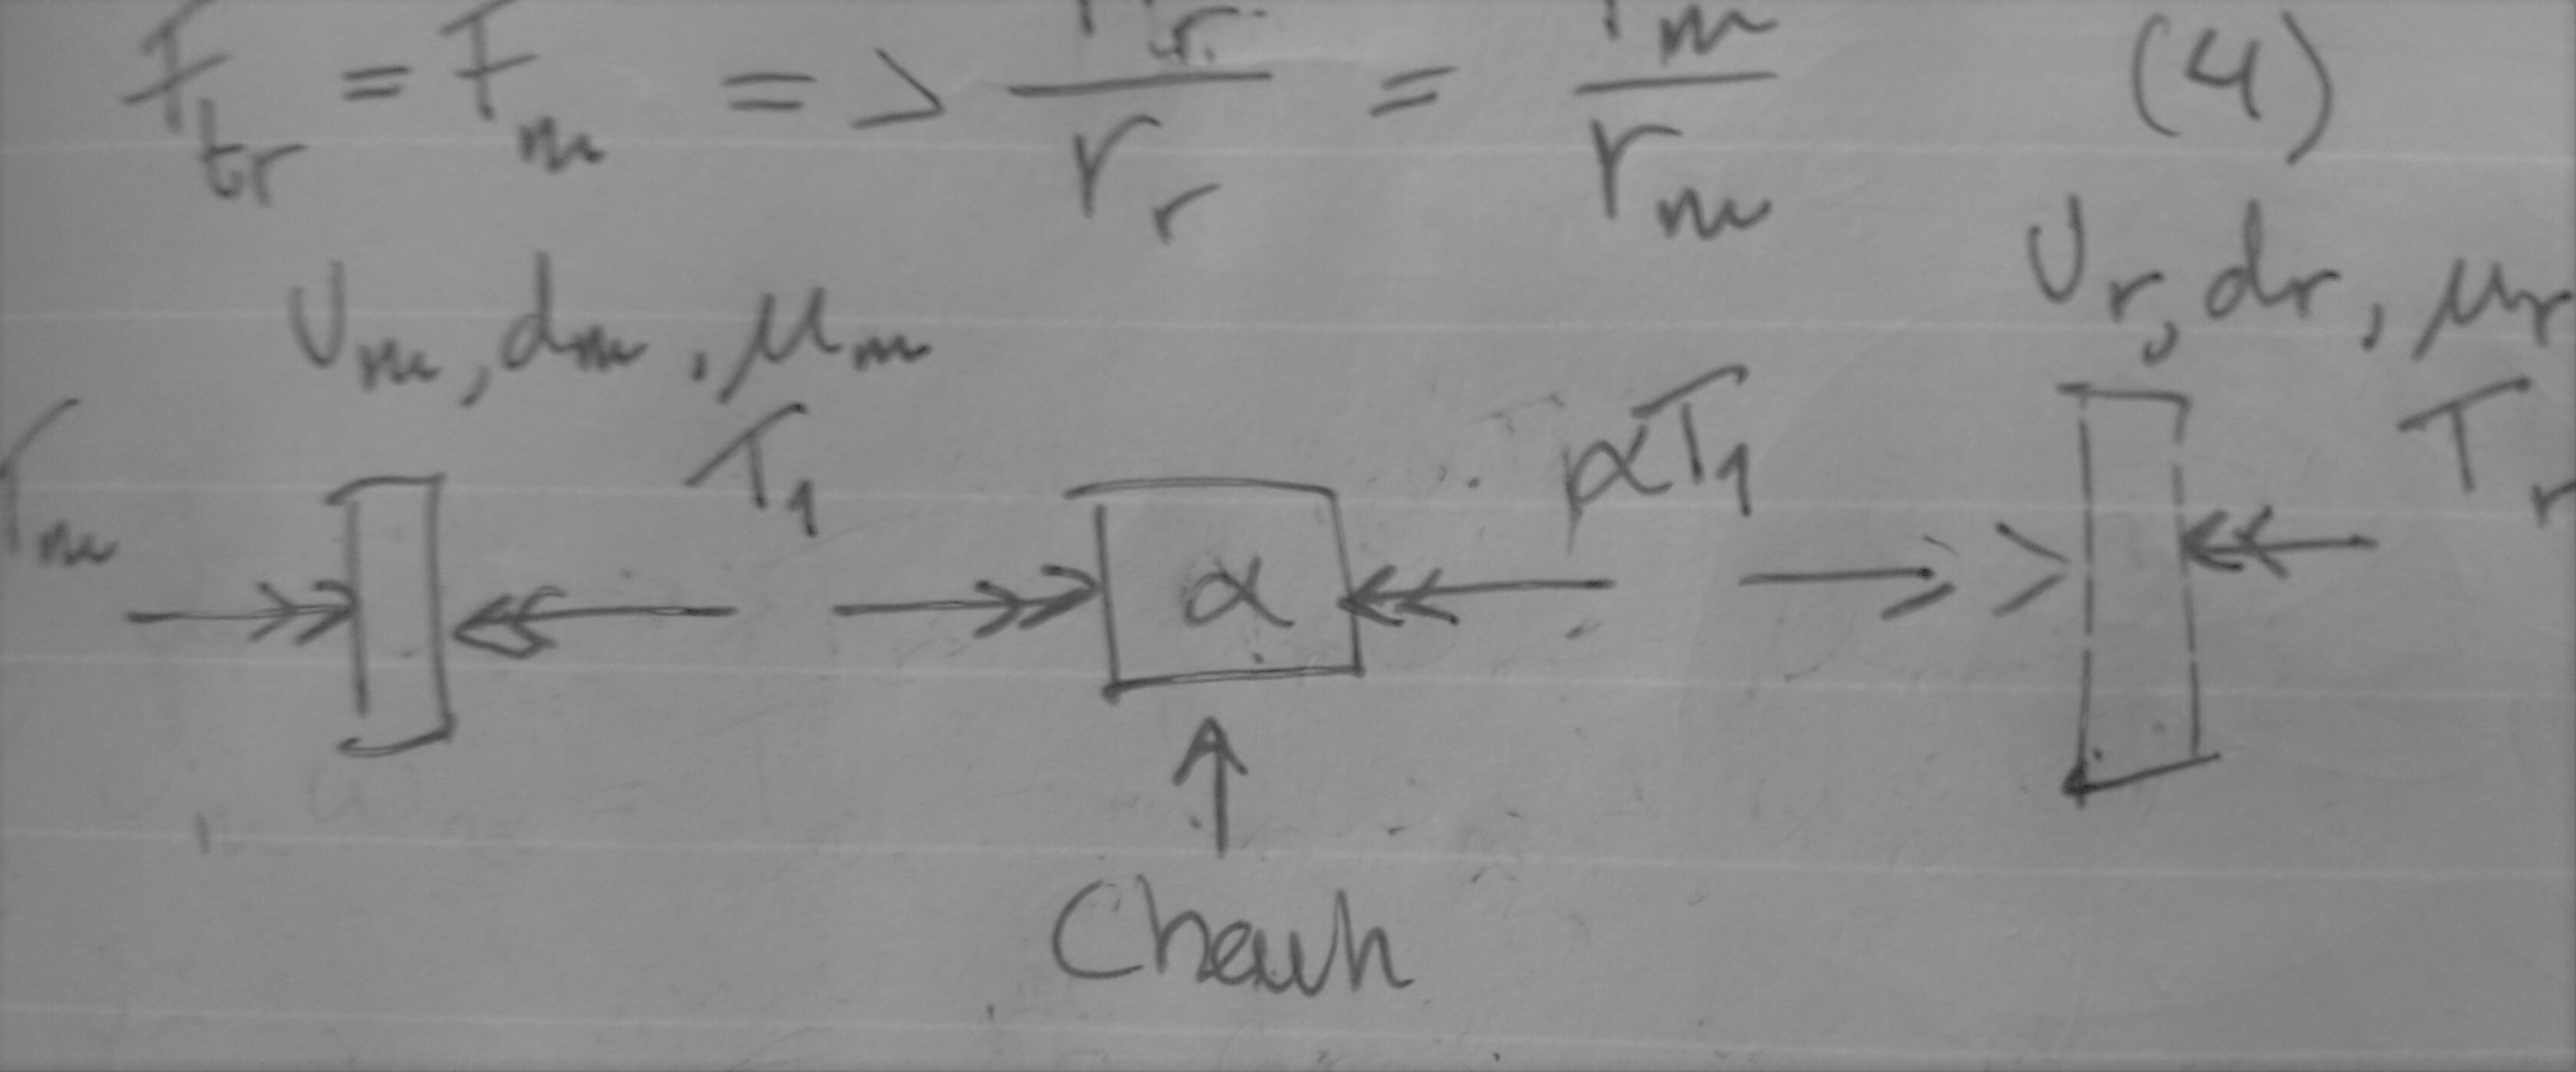
\includegraphics[width=0.9\textwidth]{./img/testrig_chaingear.png}
    \caption{Chaingear modelled as a generic gearbox with no internal friction.}
\end{figure}
This gearbox model has no internal friction.  There is always friction in a
chain gear but it is expected that this friction will be incorporated in the
total system model and the friction free representation is deemed adequate.
Using Equation (\ref{eq:testrig_rollerdynamics}) and (motor model) along with
the gearbox model, the total testrig dynamic model becomes
\begin{equation} \label{eq:testrig_totaldynamics}
    J_{tot} \dot{\omega}_m = T_m + F_{tr} r_r - d_{tot} \omega_m - \mu_{tot},
\end{equation}
with motor torque $T_m$, simulation force $F_{tr}$ and motor rotational velocity
$\omega_m$. The inertia term is the combined inertia of the motor and
roller,
\begin{equation} \label{eq:totalinertia}
    J_{tot} = J_m + J_r \frac{1} {n^2}.
\end{equation}
The friction terms are combined terms as well, namely
\begin{equation} \label{eq:testrig_totalvfric}
    d_{tot} = d_m + d_r \frac {1} {n}
\end{equation}
and
\begin{equation} \label{eq:testrig_totalfric}
    \mu_{tot} = \mu_m + \mu_r.
\end{equation}

The power $P_m$ required for the motor on the testrig is calculated as
\begin{equation} \label{eq:testrig_motorpower}
	P_m = T_m \omega_m
\end{equation}

Using the London track and the plant model of Elba, $P_m$ during one lap could be simulated, as shown in (\ref{fig:testrig_power_required}).

\begin{figure}[H]
    \label{fig:testrig_power_required}
    \centering
    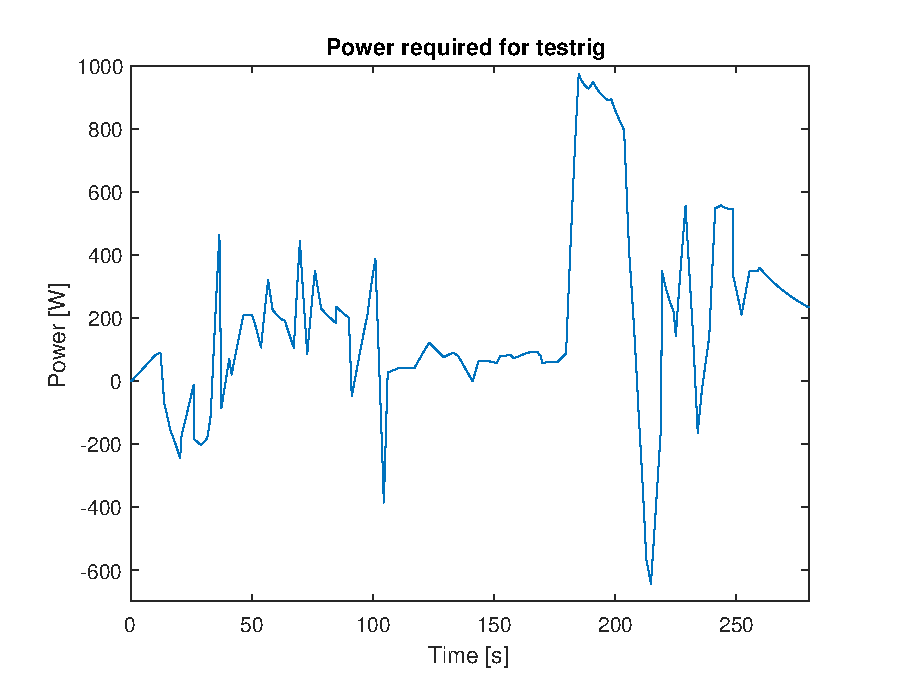
\includegraphics[width=\textwidth]{./img/testrig_power_required.eps}
    \caption{Power required for the motor on the testrig.}
\end{figure}

Figure (\ref{fig:testrig_power_required}) shows that the maximum required power from the testrig motor is $1000$ W.

\chapter{Discussion}
The purpose of this section is to give the authors thoughts and considerations
on how the different design decisions and project as a whole have turned out
with the benefit of hindsight. Not everything have been clear from the begining
and a lot of lessons have been learned along the way. The easiest way to
communicate this is to start with the project as a whole and then move into the
different parts of the project one by one. 
<<<<<<< HEAD
=======
\section{Elba}

\section{Discussion}
>>>>>>> d718bd60644eb9257f9c77dc935c02a93983054c

\subsection{Requirements}
Having good requirements gives a common goal for everyone to work towards. At
the start of the project, not much thought was given to setting requirements
first and then work towards fulfilling them. They where instead treated as
implicit to the problems to be solved and an estimation of what was acceptable
end goals where made up as we went along in the project. The lack of real
requirements led to difficulties when the projects from the other subgroups
where incorporated into the final design of the car. For example, the clutch
improvements that were made by the machine design team did not meat the
expectations of the mechatronics team i.e.\ our implicit requirements were not
the same. Had a predefined set of requirements been set up beforehand, the
consolidation and evalution of the design would have been easiier.

To make result evalutation easier, and to get a clearer definition of done,
requirements where set before work on the testrig started. There were some
difficulties with this since we were customer and the supplier, i.e.\ user and
developer. To get a clear distinction between the roles, it was decided that as
many user requirements as possible would be set with the SEM rules as a base.
Looking back, this was a good decision. We have been able to source many clear
high-level requirements from the rules, for example the requirement that the
testrig should be able to simulate the full London track. We could then sit down
as a design team and reduce the abstract user requirements to technical system
requirements. This separation of roles has helped us set fair requirements that
set demands on the system design but still allows us to create feasable
definitions of done. 

\subsection{Requirements Engineering system}
When evaluating which software to use to store the requirements, we made
special requirements for how this software should work. It was important to have
traceability, both between requirements and to who has made changes, and that
the system was easy to use. Emphasis was on an easy learning curve. Everyone in
the team has used IBM Rational Doors for requirements engineering in a previous
course, but we all found it cumbersome to use and too packed with features for
what we needed. Since only a core set of features was needed, an alternative
path was taken. Having only the essential features and being able to add new
ones as they are needed has been valuable for the team. Even though not everyone
in the team has experiance with HTML programming, the use of Markdown along with
a standard template for requirements still allow everyone to write new and edit
requirements. 

\subsection{Testrig control}
The desired output of the testrig is the combined external forces that affect
the car at any given time on a track. By construction, this means that the
output is the torque on the rollers is the desired output. Because of time
and hardware constraints, a solution where the current fed to the motor is
instead controlled. In theory, since the motor torque constant of a DC motor is
constant, the torque can be calculated by measuring the current fed to the
motor if lossses in the system are known. In practice, it is difficult to
predict losses accurately and the convoluted way of calculating the torque adds
another layer of possible errors. It also puts rather high demands on how well
the system is modeled; the torque estimation can never be better than the
accuracy of the model. An optimal solution would of course be to fit a torque
sensor to the testrig and run the system on a closed loop with current as the
control variable and torque as the output. However, under the
circumstances, the group considers the open loop current control approach to be
the best choice. Firstly, even with a lower output accuracy, it still gives a
good proof of concept of the testrig and shows that a rolling highway simulation
on Elba can be done succesfully. Secondly, a good platform for future
improvement can be built and expanded upon in future projects. It was never
feasable that a full-featured system could be designed, constructed and
implemented in such a short time scale, so it was important to build a stable
expandable platform and we consider that goal accomplished.

\subsection{Testrig identification}
As discussed in the previous section, the current control approach is not
optimal and should not be a final design for the testrig. Therefore, it has been
important to set accuracy requirements that are ´´good enough´´. A model with a
good accuracy is needed for the operation of the current setup. This allows the
concept to be proven and also lets next years team use the testrig as a tool for
getting preliminary data at the start of the project. However, spending too much
time on refining the model would be counterproductive since future versions of
the system will not be as dependent on a high accuracy model. Therefore, the
iterative approach used has been a good way of finding the right balance between
accuracy and time spent. The chosen model has obvious flaws.  Because of the
hardware setup, reliable data for the sine wave input could not be collected and
had to be roughly estimated from the settings used in the DC motor driver. This
means that the sine wave input could not be used for more than a way of
validating model behaviour instead of taking exact measurements.  It is
difficult to know weather the steady state error for the sine wave input is
because of the model or the estimation of the voltage.  It was good however to
see that the model performed well in the area where the testrig started moving
from a stand still. 

One large caveat of the parameter estimation is that it did not take measurement
noise into consideration. A big improvement on the reliability of the data could
be achieved by using the statistical methods in~\cite{modeling1994}. Usually,
measurement noise is modelled as white noise through a suitable filter. The
iterative process used in the parameter estimation could be continued to include
measurement noise. This is something that could be incorporated into further
iterations of the model identification process used, along with taking the
inductance of the motor into account. Having a flexible process with clear gates
between each model iteration has been very beneficial for the group and has
allowed us to make judgements on how much time to put on improving the models
accuracy.

Little consideration has been taken to quantization errors. The
encoder has a high resolution, 1024 pulses per revolution, which is assumed to
be high enough so that it has a small impact on the fidelity of the results.
Also, the sampling rate was set to 10 Hz. This was the highest that could be
used by Simulinks external mode to get reliable communication with the
microcontroller. It does follow the rule of thumb that the sampling rate should
be 10--30 times faster than the fastest dynamics in the system and the sampled
input and output was exact enouch so that most dynamics where rather smooth.
Both the effect of the sampling rate and the quantization of the measurements
should be investigated mathematically to determine their effect on the data.

It should be noted that having model identification as part of the project has
been very rewarding for us as students. A mechatronic engineer works in the
intersection between programming, electronics and control theory and all of
these have been used in the identification process. Control theory tells us how
model the system dynamics, we implement the measurements on an embedded system
and setup the electrical system to get the data. We have also had to use
knowledge from mechatronics subjects such as Dynamics and Motion control,
Mechatronics basic course and Embedded systems. It is this synthesis of subjects
that makes mechatronics what it is and it has been a great experience. 
\section{Conclusion}

\chapter{Future Work}
%\section{Futurework}

List of stuff to work on:

1. Separate ground between logic and power in testrig. Not possible because of the way we measure voltage. Should share logic ground with ESCON driver.

2. Map ICE parameters.

3. Improve parameters of Elba in the plant model.

4. Local optimization? Not State flow.

5. Improve clutch

6. Implement particle filter

7. Fix CAN receive from RCP to Front ECU

8. Add more interesting data to CAN msg from RCP

9. Fix instrumentation panel

10. Make the testrig to one unit i.e. mount the ECU on the testrig and make the wiring better.

11. Make the door hinges more robust\\

This list of improvements cover all of the different projects and teams that work with Elba the car. 

% Bibliography
\bibliographystyle{plain}
\bibliography{mainbib}

\chapter*{Acknowledgments}
\addcontentsline{toc}{chapter}{Acknowledgments}
There have often been a sense of distance between students and faculty staff, 
but during this project the feeling have
been the opposite, the ITM/mechatronics faculty have always been available.

\noindent
We are also grateful for our sponsors:

ITRL for sponsoring and housing the project.

SKF for providing bearings and actuators.

ECO2 and SHC for your sponsoring support.

\noindent
We also wish to thank Shell for an excellent event and the opportunity to meet our idol
Kimi Räikkönen. 

% This in not used atm
%\addtocontents{toc}{\protect\contentsline {part}{Appendices}{}{}}

\appendix
\part{Appendices}

\chapter{Vehicle Stuff}\label{appA}
%\addtocontents{toc}{\protect\contentsline {part}{Appendices}{}{}}

\section{Vehicle Networks}
CAN is a controller area newtwork ref to can stuff blaha..

\chapter{Rig Calculations}\label{app:rigdata}
This appendix contains calculations made for the test rig dynamics model. 

\section*{Drag force}
When calculating the drag force on the car, four terms must be known.
These are the air density, $\rho$, the drag coefficient $C_D$, the vertical area
$A$ and the current velocity of the vehicle, $v$~\cite{nakayama2002}. Air
density changes with atmospheric pressure and temperature, but is assumed to on
average be $1.205\si{kg/m^3}$ (\cite{nakayama2002} Table 2.2) in standard
atmospheric pressure, $1.013\si{kPa}$. 

Permissable estimations for the drag coefficient of a passenger car are
$0.28-0.37$~\cite{nakayama2002}. Elba is designed to be aerodynamically
efficient so a value in the lower regions is chosen, whereby $C_D = 0.30$ is
chosen.

Using geometrical methods, the area of Elba is estimated to $1\si{m^2}$.

Using these values in Equation (\ref{eq:testrig_csimple}), the combined air
resistance term of Elba is calculated to be $C_{tot} = 0.18$.

\chapter{Testrig software}
This section will contain information about the (new) software in the rig.

TODO\@:Encoder software (TLC)


\chapter{Elba 2015 report}\label{app:elba2015}
This appendix contains the report from the last iteration of Elba development.
Much of the information still holds true since most changes done this year are
improvements of existing systems.
%\includepdf[pages={-}]{./appendices/Elba2015.pdf}

\chapter{RaceCapture Pro 2 specifications}\label{app:RCP}
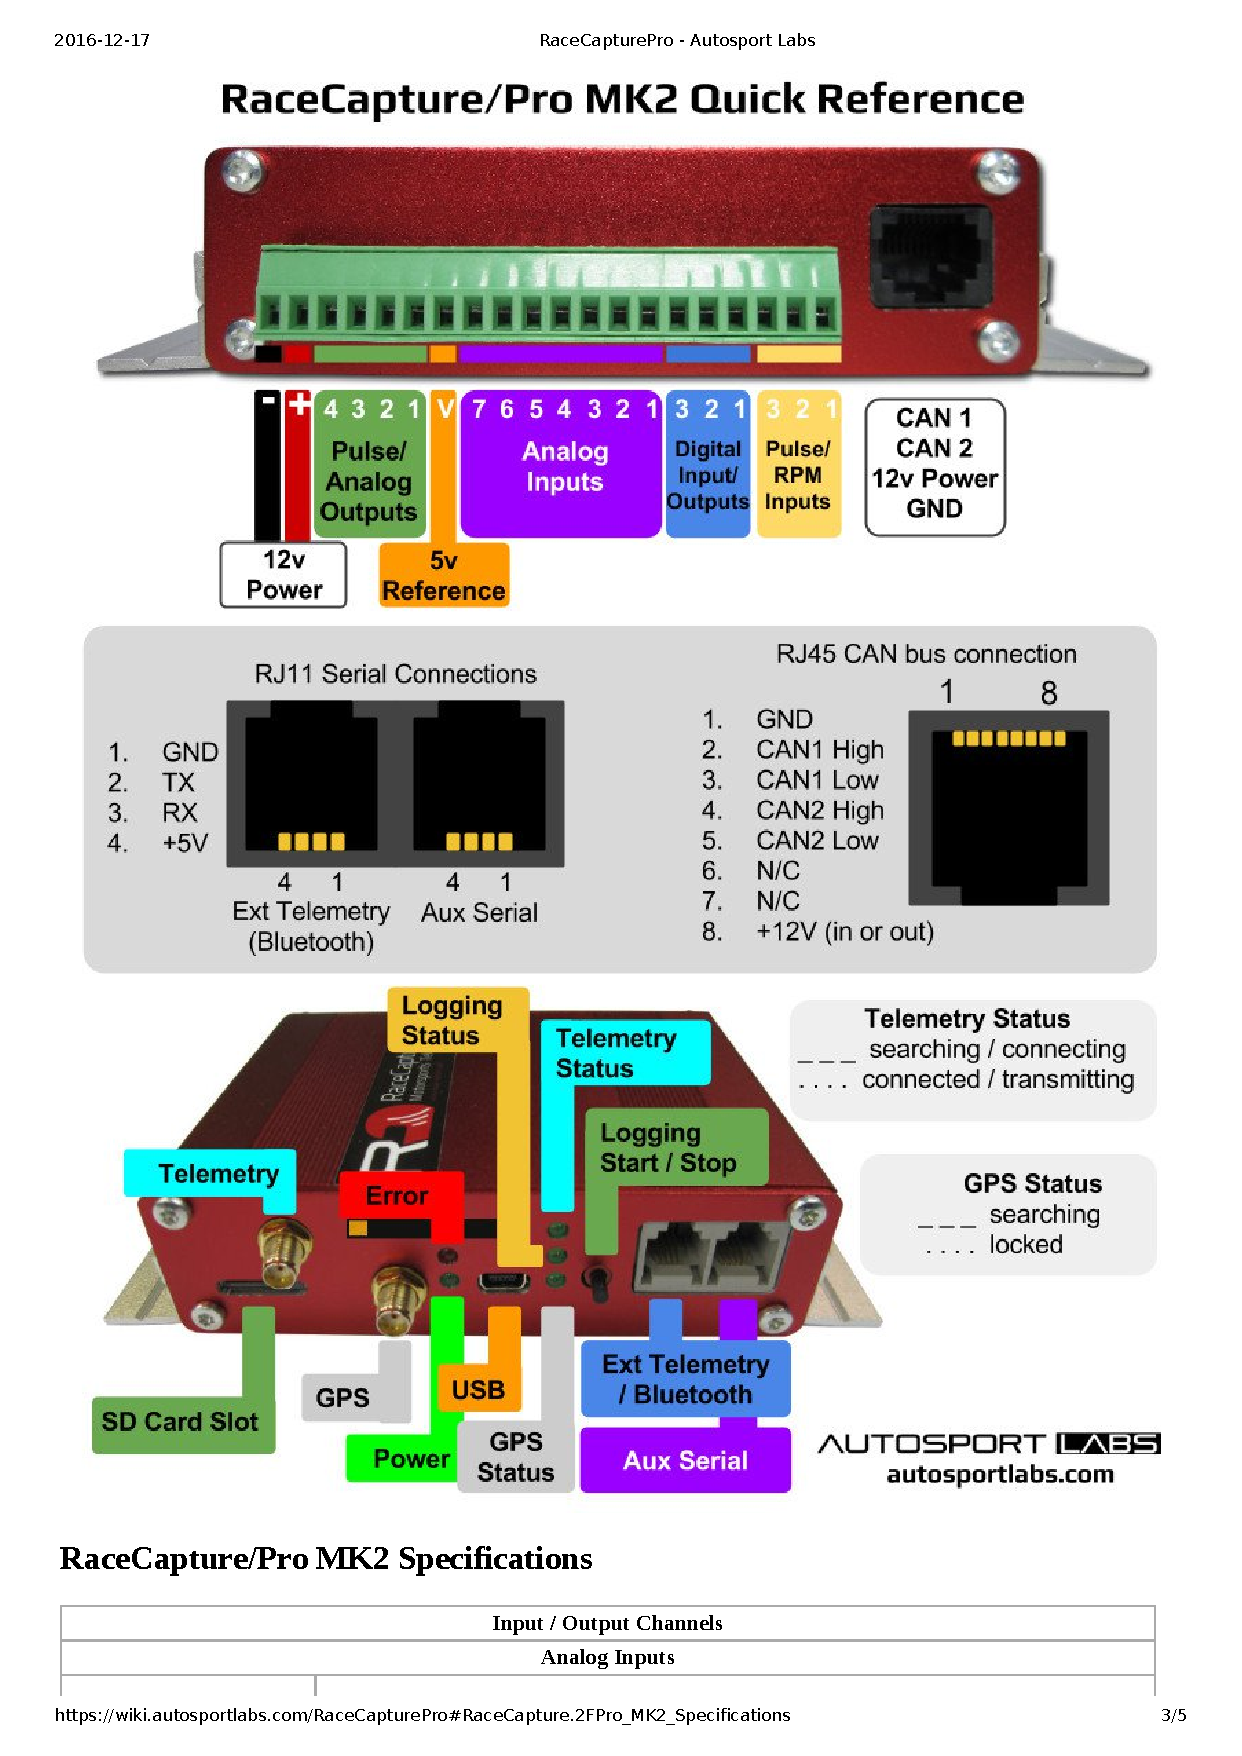
\includepdf[pages=-]{appendices/RaceCapture-Pro-MK2-quick-reference-sheet.pdf}


%% Append papers fore easy referencing, sota ice clutch
\part{Appended Papers}
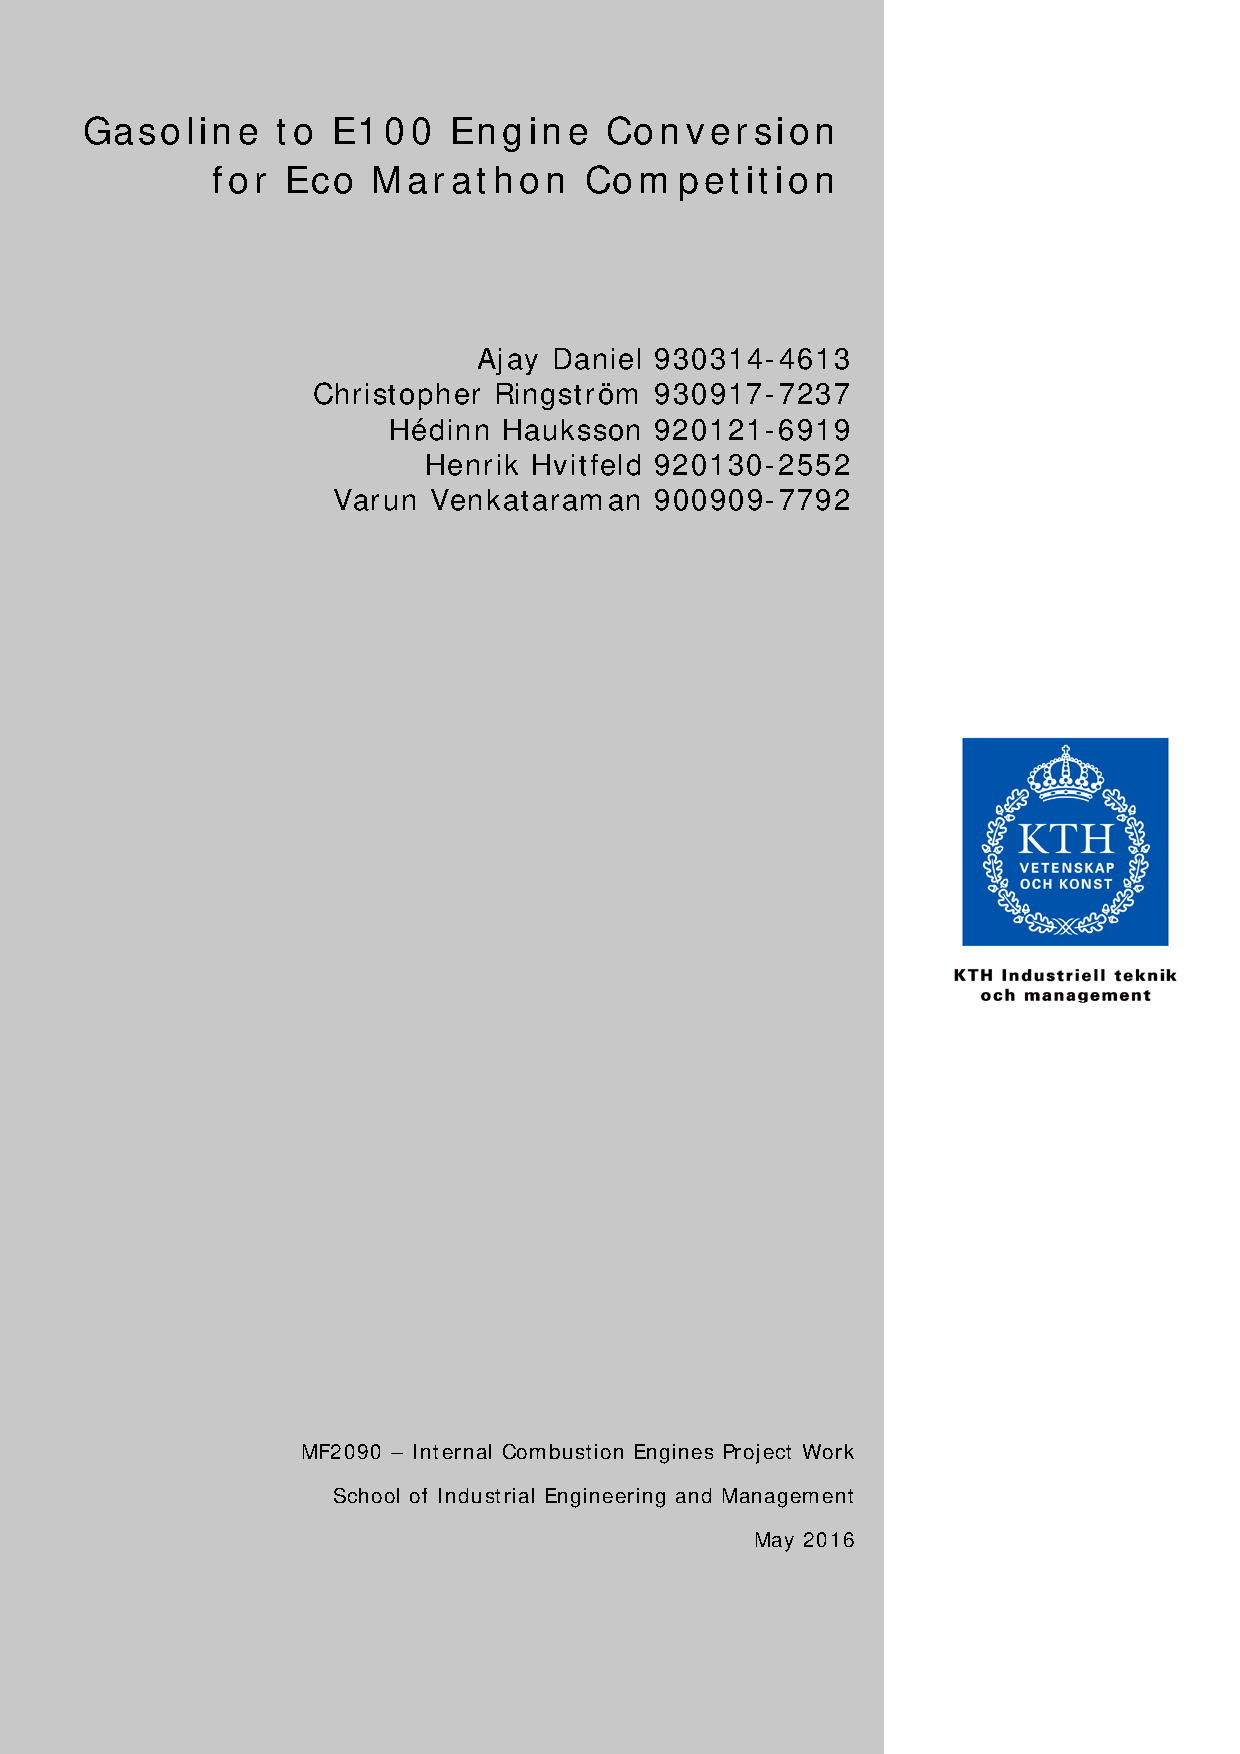
\includepdf[pages=-]{appendices/MF2090_Report_VT16.pdf}

\includepdf[pages={1-17}]{appendices/Shell_Eco_Marathon_MachineDesign.pdf}
\end{document}
